\documentclass[12pt]{article}
\usepackage[margin = 1.0in]{geometry}
\setlength{\parindent}{0in}
\usepackage{amsfonts, amssymb, amsthm, mathtools, tikz, qtree, float}
\usepackage{algpseudocode, algorithm, algorithmicx}
\usepackage{ae, aecompl, color}
\usepackage{wrapfig}
\usepackage{multicol, multicol, array}
\usepackage{imakeidx}
\makeindex[columns=2, title=Indices, intoc]

\usepackage[pdftex, pdfauthor={Charles Shen}, pdftitle={CS 350: Operating Systems}, pdfsubject={Lecture notes from CS 350: at the University of Waterloo}, pdfkeywords={course notes, notes, Waterloo, University of Waterloo}, pdfproducer={LaTeX}, pdfcreator={pdflatex}]{hyperref}
\usepackage{cleveref}

\DeclarePairedDelimiter{\set}{\lbrace}{\rbrace}
\definecolor{darkish-blue}{RGB}{25,103,185}

\hypersetup{
  colorlinks,
  citecolor=darkish-blue,
  filecolor=darkish-blue,
  linkcolor=darkish-blue,
  urlcolor=darkish-blue
}

\theoremstyle{plain}
\newtheorem{theorem}{Theorem}[subsection]

\theoremstyle{definition}
\newtheorem{proposition}[theorem]{Proposition}
\newtheorem{corollary}[theorem]{Corollary}
\newtheorem{lemma}[theorem]{Lemma}
\newtheorem{ex}[theorem]{Example}
\newtheorem*{ex*}{Example}
\newtheorem{defn}{Definition}

\crefname{ex}{Example}{Example}

\newcommand{\defnterm}[1]{\textbf{\textcolor{teal}{#1}}\index{#1}}

\newcolumntype{L}[1]{>{\raggedright\let\newline\\\arraybackslash\hspace{0pt}}m{#1}}
\newcolumntype{C}[1]{>{\centering\let\newline\\\arraybackslash\hspace{0pt}}m{#1}}
\newcolumntype{R}[1]{>{\raggedleft\let\newline\\\arraybackslash\hspace{0pt}}m{#1}}

\allowdisplaybreaks

\makeatletter
\def\blfootnote{\gdef\@thefnmark{}\@footnotetext}
\makeatother

%%%%%%%%%%%%%%%%%%%%%
%% D O C U M E N T %%
%%%%%%%%%%%%%%%%%%%%%

\begin{document}
\let\ref\Cref
\pagenumbering{roman}

\title{\bf{CS 350: Operating Systems}}
\date{Fall 2016, University of Waterloo \\ \center Notes written from Gregor Richards's lectures.}
\author{Charles Shen}

\blfootnote{Feel free to email feedback to me at
\href{mailto:ccshen902@gmail.com}{ccshen902@gmail.com}.}

\maketitle
\thispagestyle{empty}
\newpage
\tableofcontents
\newpage
\pagenumbering{arabic}

%%%%%%%%%%%%%%%%%%
%% INTRODUCTION %%
%%%%%%%%%%%%%%%%%%
\section{Introduction}
There are three views of an operating system:
\begin{enumerate}
  \item[1.] \textbf{Application View} (\ref{app_view_OS}): what service does it provide?
  \item[2.] \textbf{System View} (\ref{sys_view_OS}): what problems does it solve?
  \item[3.] \textbf{Implementation View} (\ref{impl_view_OS}): how is it built?
\end{enumerate}
\emph{An operating system is part cop, part facilitator}. \\

\textbf{kernel}: The operating system kernel is the part of the operating system that responds to system calls, interrupts and exception. \\

\textbf{operating system} (OS): The operating system as a whole includes the kernel, and may include other related programs that provide services for application such as utility programs, command interpreters, and programming libraries.

\subsection{Application View of an Operating System}\label{app_view_OS}
The OS provides an execution environment for running programs.
\begin{itemize}
  \item The execution environment provides a program with the processor time and memory space that it needs to run.
  \item The execution environment provides interfaces through which a program can use networks, storage, I/O devices, and other system hardware components. \\
  Interfaces provide a simplified, abstract view of hardware to application programs.
  \item The execution environment isolates running programs from one another and prevents undesirable interactions among them.
\end{itemize}

\subsection{System View of an Operating System}\label{sys_view_OS}
The OS manages the hardware resources of a computer system.
\begin{itemize}
  \item Resources include processors, memory, disks and other storage devices, network interfaces, I/O devices such as keyboards, mice and monitors, and so on.
  \item The operating system allocates resources among running programs. \\
  It controls the sharing of resources among programs.
  \item The OS itself also uses resources, which it must share with application programs.
\end{itemize}

\subsection{Implementation View of an Operating System}\label{impl_view_OS}
The OS is a concurrent, real-time program.
\begin{itemize}
  \item Concurrency arises naturally in an OS when it supports concurrent applications, and because it must interact directly with the hardware.
  \item Hardware interactions also impose timing constraints.
\end{itemize}

\subsection{Operating System Abstractions}
The execution environment provided by the OS includes a variety of abstract entities that can be manipulated by a running program. \\
Examples:
\begin{itemize}
  \item \textbf{files and file systems}: abstract view of secondary storage
  \item \textbf{address spaces}: abstract view of primary memory
  \item \textbf{processes, threads}: abstract view of program execution
  \item \textbf{sockets, pipes}: abstract view of network or other message channels
\end{itemize}

%%%%%%%%%%%%%%%%%%%%%%%%%%%%%
%% THREADS AND CONCURRENCY %%
%%%%%%%%%%%%%%%%%%%%%%%%%%%%%
\newpage
\section{Threads and Concurrency}
Threads provide a way for programmers to express \emph{concurrency} in a program. \\
A normal \emph{sequential program} consists of a single thread of execution. \\
In threaded concurrent programs, there are multiple threads of executions that are all occurring at the same time.

\subsection{OS/161's Thread Interface}
Create a new thread:
\begin{verbatim}
  int thread_fork(
    const char *name,             // name of new thread
    struct proc *proc,            // thread's process
    void (*func)                  // new thread's function
      (void *, unsigned long),
    void *datat1,                 // function's first param
    unsigned long data2           // function's second param
  );
\end{verbatim}

Terminating the calling thread:
\begin{verbatim}
  void thread_exit(void);
\end{verbatim}

Voluntarily yield execution:
\begin{verbatim}
  void thread_yield(void);
\end{verbatim}

\subsection{Why Threads?}
\textbf{Reason 1}: parallelism exposed by threads enables parallel execution if the underlying hardware supports it.
Programs can run faster! \\

\textbf{Reason 2}: parallelism exposed by threads enable better processor utilization. \\
If one thread has to \emph{block}, another may be able to run. \\

\textbf{Concurrent Program Execution (Two Threads)} \\
Conceptually, each thread executes sequentially using its private register contents and stack.

\subsection{Some Reviews}
\textbf{The Fetch/Execute Cycle}
\begin{enumerate}
  \item[1.] fetch instruction PC points to
  \item[2.] decode and execute instruction
  \item[3.] advance PC
\end{enumerate}

\begin{table}[H]
  \vspace{-20pt}
  \caption{MIPS Registers}
  \centering

  \begin{tabular}{|c|c|l||c|c|l|}
  \hline
  num & name & use & num & name & use \\ \hline
  0 & z0 & always zero & 24-25 & t8-t9 & temps (caller-save) \\ \hline
  1 & at & assembler reserved & 26-27 & k0-k1 & kernel temps \\ \hline
  2 & v0 & return val/syscall \# & 28 & gp & global pointer \\ \hline
  3 & v1 & return value & 29 & sp & stack pointer \\ \hline
  4-7 & a0-a3 & subroutine args & 30 & s8/fp & frame ptr (callee-save) \\ \hline
  8-15 & t0-t7 & temps (caller-save) & 31 & ra & return addr (for jal) \\ \hline
  16-23 & s0-s7 & saved (calle-save) & & &  \\ \hline
  \end{tabular}
\end{table}

\subsection{Implementing Concurrent Threads}
\textbf{Option 1}: multiple processors, multiple cores, hardware multithreading per core
\begin{itemize}
  \item $P$ processors, $C$ cores per processor, $M$ multithreading degree per core $\Rightarrow$ $P \cdot C \cdot M$ threads can execute simultaneously
  \item separate register set for each running thread, to hold its execution context
\end{itemize}
\textbf{Option 2}: \emph{timesharing}
\begin{itemize}
  \item multiple threads take turns on the same hardware
  \item rapidly switch from thread to thread so that all make progress
\end{itemize}

In practice, both techniques can be combined!

\subsection{Timesharing and Context Switches}
When timesharing, the switch from one thread to another is called a \emph{context switch}. \\

What happens during a context switch:
\begin{enumerate}
  \item[1.] decide which thread will run next (scheduling)
  \item[2.] save register contents of current thread
  \item[3.] load register contents of next thread
\end{enumerate}

Thread context must be saved/restored carefully, since thread execution continuously changes the context! \\

\textbf{Context Switch on the MIPS}
\begin{verbatim}
  switchframe_switch:
    /* a0: address of switchframe pointer of old thread. */
    /* a1: address of switchframe pointer of new thread. */
    /* Allocate stack space for saving 10 registers. 10*4 = 40 */
    addi sp, sp, -40

    sw   ra, 36(sp)  /* Save the registers */
    sw   gp, 32(sp)
    sw   s8, 28(sp)
    sw   s6, 24(sp)
    sw   s5, 20(sp)
    sw   s4, 16(sp)
    sw   s3, 12(sp)
    sw   s2, 8(sp)
    sw   s1, 4(sp)
    sw   s0, 0(sp)

    /* Store the old stack pointer in the old thread */
    sw   sp, 0(a0)

    /* Get the new stack pointer from the new thread */
    lw   sp, 0(a1)
    nop             /* delay slot for load */

    lw   s0, 0(sp)  /* Now, restore the registers */
    lw   s1, 4(sp)
    lw   s2, 8(sp)
    lw   s3, 12(sp)
    lw   s4, 16(sp)
    lw   s5, 20(sp)
    lw   s6, 24(sp)
    lw   s8, 28(sp)
    lw   gp, 32(sp)
    lw   ra, 36(sp)
    nop             /* delay slot for load */

    /* and return. */
    j ra
    addi sp, sp, 40 /* in delay slot */
    .end switchframe_switch
\end{verbatim}

\subsection{What Causes a Context Switch?}
The running thread calls \texttt{thread\_yield}, running thread \emph{voluntarily} allows other threads to run. \\
So we have the following stack (in growth order) after voluntary context switch:
\begin{itemize}
  \item thread\_yield() stack frame
  \item thread\_switch() stack frame
  \item saved thread context (switchframe)
\end{itemize}

The running thread calls \texttt{thread\_exit}, running thread is terminated. \\

The running thread \emph{blocks}, via a call to \texttt{wchan\_sleep}. \\

The running thread is \emph{preempted}, running thread \emph{involuntarily} stops running. \\
So we have the following stack (in growth order) after preemption:
\begin{itemize}
  \item trap frame
  \item interrupt handling stack frame(s)
  \item thread\_yield() stack frame
  \item thread\_switch() stack frame
  \item saved thread context (switchframe)
\end{itemize}

\begin{figure}[H]
  \centering
  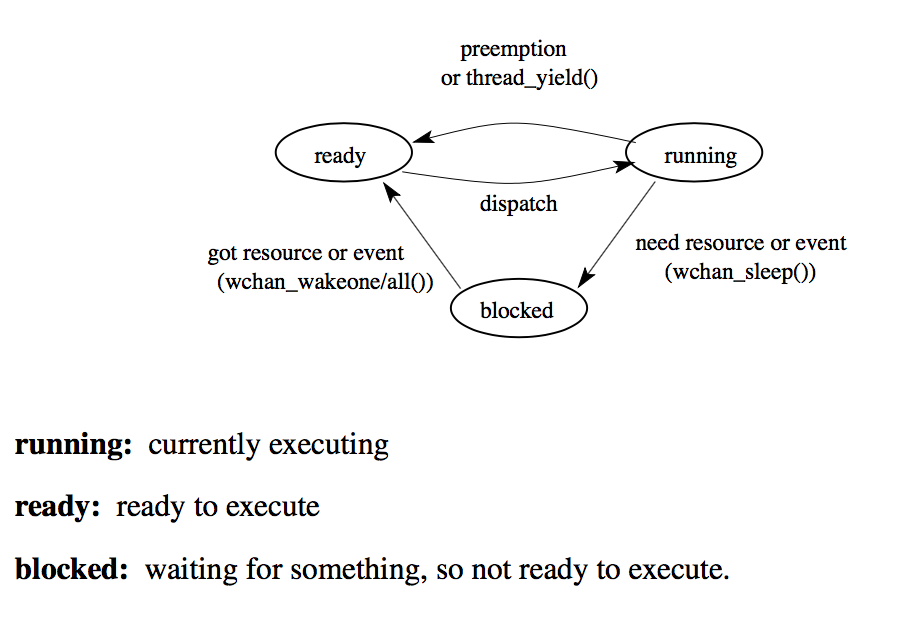
\includegraphics[scale=0.6]{pictures/thread_states.png}
  \caption{Thread States}
  \label{fig:thread_states}
\end{figure}

\subsection{Review on Interrupts}
An interrupt is an event that occurs during execution of a program. \\
Interrupts are caused by system devices (hardware), e.g., a timer, a disk controller, a network interface. \\
When an interrupt occurs, the hardware automatically transfer control to a fixed location in memory.
At that memory location, the thread library places a procedure called an \emph{interrupt handler}. \\
The interrupt handler normally:
\begin{enumerate}
  \item[1.] create a \emph{trap frame} to record thread context at the time of the interrupt
  \item[2.] determines which device caused the interrupt and performs device-specific processing
  \item[3.] restores the saved thread context from the trap frame and resumes executions of the thread
\end{enumerate}

\subsection{Preemption}
Without preemption, a running thread could potentially run forever, without yielding, blocking, or exiting. \\
\emph{Preemption} means forcing a running thread to stop running, so that another thread can have a chance. \\
To implement preemption, the thread library must have a means of ``getting control'' (causing thread library code to be executed) even though the running thread has not called a thread library function. \\
This is normally accomplished using \emph{interrupts}.

\subsubsection{Preemptive Scheduling}
A preemptive scheduler imposes a limit, called the \emph{scheduling quantum} on how long a thread can run before being preempted. \\
The quantum is an \emph{upper bound} on the amount of time that a thread can run.
It may block or yield before its quantum has expired. \\
Periodic timer interrupts allow running time to be tracked. \\
If a thread has run too long, the timer interrupt handler preempts the thread by calling \texttt{thread\_yield}. \\
The preempted thread changes state from running to ready, and it is placed on the \emph{ready queue}. \\

OS/161 threads use \emph{preemptive round-robin scheduling}.

\subsubsection{Two-Thread Example}
Thread 1 is running, thread two had previously yielded voluntarily. \\
Thread 1: program stack frame(s). \\
Thread 2: program stack frame(s), thread\_yield, thread\_switch, switch frame. \\

A time interrupt occurs. Interrupt handler runs. \\
Thread 1: program stack frame(s), trap frame, interrupt handler. \\
Thread 2: program stack frame(s), thread\_yield, thread\_switch, switch frame. \\

Interrupt handler decides THread 1 quantum has expired. \\
Thread 1: program stack frame(s), trap frame, interrupt handler, thread\_yield. \\
Thread 2: program stack frame(s), thread\_yield, thread\_switch, switch frame. \\

Scheduler chooses Thread 2 to run. Context switch. \\
Thread 1: program stack frame(s), trap frame, interrupt handler, thread\_yield, thread\_switch, switch frame. \\
Thread 2: program stack frame(s), thread\_yield, thread\_switch, switch frame. \\

Thread 2 context is restored. \\
Thread 1: program stack frame(s), trap frame, interrupt handler, thread\_yield, thread\_switch, switch frame. \\
Thread 2: program stack frame(s), thread\_yield. \\

\texttt{thread\_yield} finishes, Thread 2 program resumes. \\
Thread 1: program stack frame(s), trap frame, interrupt handler, thread\_yield, thread\_switch, switch frame. \\
Thread 2: program stack frame(s). \\

Later, Thread 2 yields again. Scheduler chooses Thread 1. \\
Thread 1: program stack frame(s), trap frame, interrupt handler, thread\_yield, thread\_switch, switch frame. \\
Thread 2: program stack frame(s), thread\_yield, thread\_switch, switch frame. \\

Thread 1 context is restored, interrupt handler resumes. \\
Thread 1: program stack frame(s), trap frame, interrupt handler. \\
Thread 2: program stack frame(s), thread\_yield, thread\_switch, switch frame. \\

Interrupt handler restores state from trap frame and returns. \\
Thread 1: program stack frame(s). \\
Thread 2: program stack frame(s), thread\_yield, thread\_switch, switch frame.


%%%%%%%%%%%%%%%%%%%%%
%% SYNCHRONIZATION %%
%%%%%%%%%%%%%%%%%%%%%
\newpage
\section{Synchronization}
\subsection{Thread Synchronization}
All threads in a concurrent program \emph{share access} to the program's global variables and the heap. \\
The part of a concurrent program in which a shared object is accessed is called a \emph{critical section}. \\

\texttt{volatile} keyword:
Without it, the compiler could optimize the code on the variable. \\
\texttt{volatile} forces the compiler to load and store the value on every use.
Otherwise, we may have a variable that is loaded before a loop and stored after the loop terminates which may not be what we want/expect.

\subsection{Mutual Exclusion}
To prevent race conditions, we can enforce \emph{mutual exclusion} on critical sections in the code. \\

A \emph{race condition} is an undesirable situation that occurs when a device or system attempts to perform two or more operations at the same time, but because of the nature of the device or system, the operations must be done in the proper sequence to be done correctly.

\subsubsection{Enforcing Mutual Exclusions With Locks}
Acquire/Release must ensure that only one thread at a time can hold the lock, even if both attempt to Acquire at the same time. \\
If a thread cannot Acquire the lock immediately, it must wait until the lock is available.

\subsection{Hardware-Specific Synchronization Instructions}
Used to implement synchronization primitives like locks. \\
Provide a way to \emph{test and set} a lock in a single \emph{atomic} (indivisible) operation.
\begin{ex*}
x86 \texttt{xchg} instruction:
\begin{verbatim}
  xchg  src, addr
\end{verbatim}
where \texttt{src} is typically a register, and \texttt{addr} is a memory address. \\
Value in register \texttt{src} is written to memory at address \texttt{addr}, and the old value at \texttt{addr} is placed into \texttt{src}.
\end{ex*}
Logical behaviour of \texttt{xchg} can be thought of as an \emph{atomic} function that behaves like this:
\begin{verbatim}
  Xchg(value,addr) {
    old = *addr;
    *addr = value;
    return(old);
  }
\end{verbatim}

\subsubsection{Lock Acquire and Release with Xchg}
\begin{verbatim}
  Acquire(bool *lock) {
    while (Xchg(true,lock) == true) ;
  }
  Release(book *lock) {
    *lock = false; /* give up the lock */
  }
\end{verbatim}
If \texttt{Xchg} returns \texttt{true}, the lock was already set, and we must continue to loop. \\
If \texttt{Xchg} returns \texttt{false}, then the lock was free, and we have now acquired it. \\

This construct is known as a \emph{spin lock}, since a thread busy-waits (loops) in Acquire until the lock is free!

\subsubsection{Other Synchronization Instructions}
SPARC \texttt{cas} instruction
\begin{verbatim}
  cas   addr, R1, R2
\end{verbatim}
if value at \texttt{addr} matches value in \texttt{R1} then swap contents of \texttt{addr} and \texttt{R2}. \\

Compare-And-Swap
\begin{verbatim}
  CompareAndSwap(addr, expectedval, newval)
    old = *addr;            // get old value at addr
    if (old == expectedval)
      *addr = newval;
    return old;
\end{verbatim}

MIPS load-linked and store-conditional \\
Load-linked returns the current value of a memory location, while a subsequent store-conditional to the same memory location will store a new value only if no updates have occurred to that location since the load-linked.

\subsection{Spinlocks in OS/1616}
\begin{verbatim}
  struct spinlock {
    volatile spinlock_data_t lk_lock;
    struct cpu *lk_holder;
  };
  void spinlock_init(struct spinlock *lk);
  void spinlock_acquire(struct spinlock *lk);
  void spinlock_release(struct spinlock *lk);
\end{verbatim}
\texttt{spinlock\_acquire} calls \texttt{spinlock\_data\_testandset} in a loop until the lock is acquired. \\
Using Load-Linked/Store-Conditional:
\begin{verbatim}
  /* return value 0 indicates lock was acquired */
  spinlock_data_testandset(volatile spinlock_data_t *sd) {
    spinlock_data_t x,y;
    y = 1;
    __asm volatile(
      ".set push;"      /* save assembler mode */
      ".set mips32;"    /* allow MIPS32 instructions */
      ".set volatile;"  /* avoid unwanted optimization */
      "ll %0, 0(%2);"   /* x = *sd */
      "sc %1, 0(%2);"   /* *sd = y; y = success? */
      ".set pop"        /* restore assembler mode */
      : "=r" (x), "+r" (y) : "r" (sd));
    if (y == 0) { return 1; }
    return x;
  }
\end{verbatim}

\subsection{OS/161 Locks}
In addition to spinlocks, OS/161 also has \emph{locks}. \\
Like spinlocks, locks are used to enforce mutual exclusion.
\begin{verbatim}
  struct lock *mylock = lock_create("LockName");

  lock_acquire(mylock);
    critical section
  lock_release(mylock);
\end{verbatim}

Spinlock \emph{spins}, locks \emph{blocks}:
\begin{itemize}
  \item a thread that calls \texttt{spinlock\_acquire} spins until the lock can be acquired
  \item a thread that called \texttt{lock\_acquire} \emph{blocks} until the lock can be acquired
\end{itemize}

\subsection{Thread Blocking}
Sometimes a thread will need to wait for something, e.g.:
\begin{itemize}
  \item wait for a lock to be released by another thread
  \item wait for data from a (relatively) slow device
  \item wait for input from a keyboard
  \item wait for busy device to become idle
\end{itemize}

When a thread blocks, it stops running:
\begin{enumerate}
  \item[i.] the scheduler chooses a new thread to run
  \item[ii.] a context switch from the blocking thread to the new thread occurs
  \item[iii.] the blocking thread is queued in a \emph{wait queue} (not on the ready list)
\end{enumerate}

Eventually, a blocked thread is signalled and awakened by another thread.

\subsection{Wait Channels in OS/161}
Wait channels are used to implement thread blocking in OS/161.
\begin{itemize}
  \item \texttt{void wchan\_sleep (struct wchan *wc);} \\
  blocks calling thread on wait channel \texttt{wc} \\
  causes a context switch, like \texttt{thread\_yield}
  \item \texttt{void wchan\_wakeall (struct wchan *wc);} \\
  unblocks all threads sleeping on waiting channel \texttt{wc}
  \item \texttt{void wchan\_wakeone (struct wchan *wc);} \\
  unblocks one thread sleeping on waiting channel \texttt{wc}
  \item \texttt{void wchan\_lock (struct wchan *wc);} \\
  prevent operations on wait channel \texttt{wc}
\end{itemize}
There can be many different wait channels, holding threads that are blocked for different reasons. \\

Ready threads are queued on the ready queue, blocked threads are queued on wait channels (refer to \ref{fig:thread_states}).

\subsection{Semaphores}
A semaphore is a synchronization primitive that can be used to enforce mutual exclusion requirements.
It can also be used to solve other kinds of synchronization problems. \\

A semaphore is an object that has an integer value, and that supports two operations (\emph{atomic} by definition):
\begin{itemize}
  \item[\textbf{P}:] if the semaphore value is greater than 0, decrement the value. \\
  Otherwise, wait until the value is greater than 0 and then decrement it.
  \item[\textbf{V}:] increment the value of the semaphore
\end{itemize}

\subsection{Condition Variables in OS/161}
Each cv is purposed to work together along with a lock: cvs are used \emph{from within the critical section protected by the lock}. \\
Supported operations:
\begin{itemize}
  \item[\textbf{wait}:] causes calling thread to block, and it releases the lock associated within the cv. \\
  Once the thread is unblocked, it reacquires the lock.
  \item[\textbf{signal}:] one of the threads blocked on the signalled cv is unblocked
  \item[\textbf{broadcast}:] all threads blocked on the cv are unblocked
\end{itemize}

\subsubsection{Using Condition Variables}
Cvs allow threads to wait for arbitrary conditions to become true inside of a critical section. \\
By convention, each cv corresponds to a particular condition of interest to an application. \\
When a condition is not true, a thread can \texttt{wait} on the corresponding cv until it becomes true. \\
When a thread detects that a condition is true, it uses \texttt{signal} or \texttt{broadcast} to notify any threads that may be waiting. \\

Note: signalling (or broadcasting to) a cv that has no waiting threads has \emph{no effect}.
Signals \emph{do not} accumulate.

\subsubsection{Waiting on Condition Variables}
The OS/161 condition variables follows the Mesa-style condition variables. \\
When a blocked thread is unblocked, it reacquires the lock before returning from the \texttt{wait} call. \\
A thread is in the critical section when it calls \texttt{wait}, and it will be in the critical section when \texttt{wait} returns.
In between the call and the return, while the caller is blocked, the caller is \emph{out} of the critical section, and other threads may enter! \\
The thread that calls \texttt{signal} (or \texttt{broadcast}) to wake up the waiting thread will itself be in the critical section when it signals.
The waiting threads need to wait until the signaller releases the lock before it unblocks and return from the \texttt{wait} call.

\subsubsection{Example}
\begin{verbatim}
  int volatile count = 0;
  struct lock *mutex;
  struct cv *notfull, *notempty;
  /* Initialization Note: the lock and cv's must be created
   * using lock_create() and cv_create() before Produce()
   * and Consume() are called
   */
  Produce(itemType item) {            itemType Consume() {
    lock acquire(mutex);                lock_acquire(mutex);
    while (count == N) {                while (count == 0)
      cv_wait(notfull, mutex);            cv_wait(nonempty, mutex);
    }                                   remove item from buffer
    add item to buffer                  count = count - 1;
    count = count + 1;                  cv_signal(notfull, mutex);
    cv_signal(notempty, mutex);         lock_release(mutex);
    lock release(mutex);                return(item);
  }                                   }
\end{verbatim}

\subsection{Deadlocks}
Threads are \emph{deadlocked} when none of the threads can make progress (i.e. waiting on a lock indefinitely). \\
Waiting does not resolve the deadlock. \\
Those threads are permanently stuck.

\subsubsection{Two Techniques for Deadlock Prevention}
\textbf{No Hold and Wait}:
prevent a thread from requesting resources if it currently has resources allocated to it. \\
A thread may hold several resources, but to do so it must make a single request for all of them. \\

\textbf{Resource Ordering}:
Order the resource types, and require that each thread acquire resources in increasing resource type order. \\
That is, a thread may make no request for resources of type less than or equal to $i$ if it is holding resources of type $i$.


%%%%%%%%%%%%%%%%%%%%%%%%%%%%%%%%
%% PROCESSES AND SYSTEM CALLS %%
%%%%%%%%%%%%%%%%%%%%%%%%%%%%%%%%
\newpage
\section{Processes and System Calls}
\subsection{What is a Process?}
A \emph{process} is an environment in which an application program runs. \\
A process includes virtualized \emph{resources} that its program can use:
\begin{itemize}
  \item one (or more) threads
  \item virtual memory, used for the program's code and data
  \item other resources
\end{itemize}
Processes are created and managed by the \emph{kernel}. \\
Each program's process \emph{isolates} it from other programs in other processes.

\subsection{System Calls}
System calls (syscalls) are the interface between processes and the kernel. \\
A process uses syscalls to request operating system services.
\begin{table}[H]
  \vspace{-20pt}
  \caption{Syscall examples}
  \label{tab:ex_syscall}
  \centering
  \begin{tabular}{c|l}
  Services & OS/161 Examples \\ \hline
  create, destroy, manage processes & \texttt{fork, execv, waitpid, getpid} \\
  create, destroy, read, write files & \texttt{open, close, remove, read, write} \\
  manage file system and directories & \texttt{mkdir, rmdir, link, sync} \\
  interprocess communication & \texttt{pipe, read, write} \\
  manage virtual memory & \texttt{sbrk} \\
  query, manage system & \texttt{reboot, \_time}
  \end{tabular}
\end{table}

\subsection{Kernel Privilege}
Kernel code runs at a higher level of \emph{execution privilege} than application code. \\
Privilege levels are implemented by the CPU. \\

The kernel's higher privilege level allows it to do things that the CPU prevents less-privileged (application) programs from doing, like
\begin{itemize}
  \item application programs cannot modify the page tables that the kernel uses to implement process virtual memories
  \item application programs cannot halt the CPU
\end{itemize}

These restrictions allow the kernel to keep processes isolated from one another --- and from the kernel. \\

\textbf{Note}: application programs cannot directly call kernel functions or access kernel data structures.

\subsection{How System Calls Work}
There are only \emph{two} things that make kernel code run! \\

On the MIPS, the same mechanism handles exceptions and interrupts, and there is a single handler for both in the kernel.
The handler uses these codes to determine what triggered it to run.

\subsubsection{Interrupts}
Interrupts are generated by devices. \\
An interrupt means a device (hardware) needs attention. \\

Recall that an interrupt causes the hardware to transfer control to a fixed location in
memory, where an \emph{interrupt handler} is located. \\

Interrupt handlers are part of the kernel. \\
If an interrupt occurs while an application program is running, control will jump from the application to the kernel's interrupt handler. \\

When an interrupt occurs, the processor switches to privileged execution mode when it transfers control to the interrupt handler.
This is how the kernel gets its execution privilege.

\subsubsection{Exceptions}
Exceptions are caused by instruction execution. \\
An exception means that a running program needs attention. \\

Exceptions are conditions that occur during the execution of a program instruction. \\
Examples: arithmetic overflows, illegal instructions, or page faults. \\

Exceptions are detected by the CPU during instruction execution. \\

The CPU handles exceptions like it handles interrupts:
\begin{itemize}
  \item control is transferred to a fixed location, where an \emph{exception handler} is located
  \item the processor is switched to privileged execution mode
\end{itemize}
The exception handler is part of the kernel \\

\textbf{MIPS Exception Types}:
\begin{verbatim}
  EX_IRQ    0     /* Interrupt */
  EX_MOD    1     /* TLB Modify (write to read-only page) */
  EX_TLBL   2     /* TLB miss on load */
  EX_TLBS   3     /* TLB miss on store */
  EX_ADEL   4     /* Address error on load */
  EX_ADES   5     /* Address error on store */
  EX_IBE    6     /* Bus error on instruction fetch */
  EX_DBE    7     /* Bus error on data load *or* store */
  EX_SYS    8     /* Syscall */
  EX_BP     9     /* Breakpoint */
  EX_RI     10    /* Reserved (illegal) instruction */
  EX_CPU    11    /* Coprocessor unusable */
  EX_OVF    12    /* Arithmetic overflow */
\end{verbatim}

\subsubsection{Performing a Syscall}
To perform a syscall, the application program needs to cause an exception to make the kernel execute! \\
The kernel's exception handler checks the exception code (set by the CPU when the exception is generated) to distinguish syscall exceptions from other types of exceptions. \\

On the MIPS, \texttt{EX\_SYS} is the syscall exception. \\
To cause this exception on the MIPS, the application executes a special purpose instruction: \texttt{syscall}.
Other processor instruction sets include similar instructions, e.g., \texttt{syscall} on x86.

\subsubsection{System Call Timeline}
\begin{figure}[H]
  \centering
  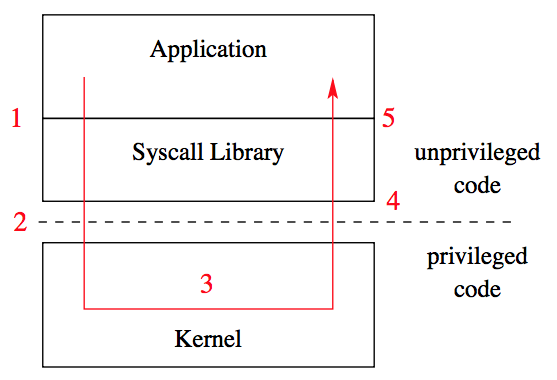
\includegraphics[scale=0.39]{pictures/syscall_stack.png}
  \caption{System call software stack}
  \label{fig:syscall_stack}
\end{figure}
\begin{enumerate}
  \item[1.] application calls library wrapper function for desired system call
  \item[2.] library function performs \texttt{syscall} instruction
  \item[3.] kernel exception handler runs
  \begin{itemize}
    \item creates a trap frame to save application program state
    \item determines that this is a syscall exception
    \item determines which syscall is being requested
    \item does the work for the requested system call
    \item restores the application program state from the trap frame
    \item returns from the exception
  \end{itemize}
  \item[4.] library wrapper function finishes and returns from its call
  \item[5.] application continues execution
\end{enumerate}

\subsubsection{Which Syscall?}
The kernel uses system call codes to determine which syscall the application is requesting,
\begin{itemize}
  \item the kernel defines a code for each syscall it understands
  \item the kernel expects the application to place a code in a specified location before executing the \texttt{syscall} instruction. \\
  For OS/161 on the MIPS, the code goes in register \texttt{v2}
  \item the kernel's exception handler checks this code to determine which system call has been requested
  \item the codes and and code location are part of the \emph{kernel ABI} (Application Binary Interface)
\end{itemize}

\subsubsection{Syscall Parameters}
The application places parameter values in kernel-specified locations before the \texttt{syscall}, and looks for return values in kernel-specified locations after the exception handler returns,
\begin{itemize}
  \item The locations are part of the kernel ABI
  \item Parameter and return value placement is handled by the application system call library functions
  \item On the MIPS
  \begin{itemize}
    \item parameters go in registers \texttt{a0, a1, a2, a3}
    \item result success/fail code is in \texttt{a3} on return
    \item return value or error code is in \texttt{v0} on return
  \end{itemize}
\end{itemize}

\subsection{User and Kernel Stacks}
Every OS/161 process thread has two stacks, although it only uses one at a time. \\

\textbf{User (Application) Stack}: used while application code is executing,
\begin{itemize}
  \item this stack is located in the application's virtual memory
  \item it holds activation records for application functions
  \item the kernel creates this stack when it sets up the virtual address memory for the process
\end{itemize}

\textbf{Kernel Stack}: used while the thread is executing kernel code, after an exception or interrupt,
\begin{itemize}
  \item this stack is a kernel structure
  \item in OS/161, the \texttt{t\_stack} field of the \texttt{thread} structure points to this stack
  \item this stack holds activation records for kernel functions
  \item this stack also holds \emph{trap frames} and \emph{switch frames} (because the kernel creates trap frames and switch frames)
\end{itemize}

\subsection{Exception Handling in OS/161}
First to run is careful assembly code that
\begin{itemize}
  \item saves the application stack pointer
  \item switches the stack pointer to point to the thread's kernel stack
  \item carefully saves application state and the address of the instruction that was interrupted in a trap frame on the thread's kernel stack
  \item calls \texttt{mips\_trap}, passing a pointer to the trap frame as a parameter
\end{itemize}

After \texttt{mips\_trap} is finished, the handler will
\begin{itemize}
  \item restore application state (including the application stack pointer) from the trap frame on the thread's kernel stack
  \item jump back to the application instruction that was interrupted, and switch back to unprivileged execution mode
\end{itemize}

\subsubsection{mips\_trap}
\texttt{mips\_trap} determines what type of exception this is by looking at the exception code. \\
There is a separate handler in the kernel for each type of exception:
\begin{itemize}
  \item interrupt? call \texttt{mainbus\_interrupt}
  \item address translation exception? call \texttt{vm\_fault}
  \item system call? call \texttt{syscall} (kernel function), passing it the trap frame pointer
\end{itemize}

\subsection{Multiprocessing}
Multiprocessing (or multitasking) means having multiple processes existing at the same time. \\

All processes share the available hardware resources, with the sharing coordinated by the OS:
\begin{itemize}
  \item Each process' virtual memory is implemented using some of the available physical memory. \\
  The OS decides how much memory each process gets.
  \item Each process' threads are scheduled onto the available CPUs (or CPU cores) by the OS.
  \item Processes share access to other resources (e.g., disks, network devices, I/O devices) by making syscalls. \\
  The OS controls this sharing.
\end{itemize}

The OS ensures that processes are isolated from one another. \\
Interprocess communication should be possible, but only at the explicit request of the processes involved.

\begin{table}[H]
  \vspace{-15pt}
  \caption{Syscalls for Process Management}
  \label{tab:syscall_pmanage}
  \centering

  \begin{tabular}{|c||c|c|}
  \hline
  & Linux & OS/161 \\ \hline
  Creation & \texttt{fork, execv} & \texttt{fork, execv} \\ \hline
  Destruction & \texttt{\_exit, kill} & \texttt{\_exit} \\ \hline
  Synchronization & \texttt{wait, waitpid, pause, ...} & \texttt{waitpid} \\ \hline
  Attribute Mgmt & \texttt{getpid, getuid, nice, getrusage, ...} & \texttt{getpid} \\ \hline
  \end{tabular}
\end{table}

\subsection{\texttt{fork}, \texttt{\_exit}, and \texttt{waitpid}}
\texttt{fork} creates a new process (the \emph{child}) that is a clone of the original (the \emph{parent}),
\begin{itemize}
  \item after \texttt{fork}, both parent and child are executing copies of the same program
  \item virtual memories of parent and child are identical at the time of the fork, but may diverge afterwards
  \item \texttt{fork} is called by the parent, but returns in \emph{both} the parent and the child! \\
  Parent and child see different return values from \texttt{fork}, parent gets child's pid and child gets 0.
\end{itemize}

\texttt{\_exit} terminates the process that calls it,
\begin{itemize}
  \item process can supply an exit status code when it exits
  \item kernel records the exit status code in case another process asks for it (via \texttt{waitpid})
\end{itemize}

\texttt{waitpid} lets a process wait for another to terminate, and retrieve its exit status code.

\subsection{The \texttt{execv} system call}
\texttt{execv} changes the program that a process is running. \\
The calling process's current virtual memory is destroyed. \\
The process gets a new virtual memory, initialized with the code and data of the new program to run. \\
After \texttt{execv}, the new program starts executing.

%%%%%%%%%%%%%%%%%%%%%%%%%%
%% ASSIGNMENT 2A REVIEW %%
%%%%%%%%%%%%%%%%%%%%%%%%%%
\newpage
\section{Assignment 2A Review}
\subsection{\texttt{fork}}
\begin{enumerate}
  \item[i.] Create process structure for child process. \\
  Use \texttt{proc\_create\_runprogram} to create the process structure, sets up the VFS and console.
  \item[ii.] Create and copy address space (and data) from parent to child. \\
  Child process must be identical to the parent process. \\
  \texttt{as\_copy} creates a new address space, and copies the pages from the old address space to the new one. \\
  Address space is not associated with the new process yet.
  \item[iii.] Attach the newly created address space to the child process structure.
  \item[iv.] Assign PID to child process and create the parent/child relationship. \\
  PIDs should be unique (no two processes should have the same PID). \\
  PIDs should be reusable.
  \item[v.] Create thread for child process (need a safe way to pass the trapframe to the child thread). \\
  Use \texttt{thread\_fork} to create a new thread. \\
  Need to pass trapframe to the child thread.
  \item[vi.] Child thread needs to put the trapframe onto the stack and modify it so that it returns the current value (and executes the next instruction)
  \item[vii.] Call \texttt{mips\_usermode} in the child to go back to userspace
\end{enumerate}

\textbf{Note}: need to ensure that the new thread does not go to user mode until its address space and trap frame have been set up (requires synchronization)!
In addition, the parent process must not return to user mode until its address space and trap frame have been copied.

\subsection{\texttt{waitpid}}
Only the parent can call \texttt{waitpid} on its children. \\
If \texttt{waitpid} is called before the child process exits, then the parent must wait/block. \\
If \texttt{waitpid} is called after the child process has exited, then the parent should immediately get the exit status and exit code. \\
PID cleanup should not rely on \texttt{waitpid}.
Parent process is not guaranteed to call \texttt{waitpid} when it exits.

\subsection{\texttt{getpid}}
Returns the PID of the current process. \\
Need to perform process assignment even without/before any fork calls.
The first user process might call \texttt{getpid} before creating any children.
\texttt{getpid} needs to return a valid PID for this process.

\subsection{\texttt{\_exit}}
Causes the current process to exit. \\
Exit code is passed to the parent process.

%%%%%%%%%%%%%%%%%%%%%%%%%%
%% ASSIGNMENT 2B REVIEW %%
%%%%%%%%%%%%%%%%%%%%%%%%%%
\newpage
\section{Assignment 2B Review}
\texttt{int execv (const char* program, char** args);} \\

Replaces currently executing program with a newly loaded program image. \\
Process id remains unchanged. \\
Path of the program is passed in as \texttt{program}. \\
Arguments to the program (\texttt{args}) is an array of \texttt{NULL} terminated strings. \\
The array is terminated by a \texttt{NULL} pointer. \\
In the new user program, \texttt{argv[argc]} should \texttt{== NULL}.

\subsection{\texttt{runprogram}}
\texttt{execv} is very similar to \texttt{runprogram} \\
\texttt{runprogram} is used to load and execute the first program from the \texttt{menu},
\begin{enumerate}
  \item[1.] Opens the program file using \texttt{vfs\_open(progname, ...)}
  \item[2.] Creates a new address space (\texttt{as\_create}), switches the process to that address space (\texttt{curproc\_setas}) and then activate it (\texttt{as\_activate})
  \item[3.] Using the opened program file, load the program image using \texttt{load\_elf}
  \item[4.] Define the user stack using \texttt{as\_define\_stack}
  \item[5.] Call \texttt{enter\_new\_process} with no parameters, the stack pointer (determined by \texttt{as\_define\_stack}) \emph{and} entry point for the executable (determined by \texttt{load\_elf})
\end{enumerate}

\subsection{\texttt{execv}}
\begin{itemize}
  \item Count the number of arguments and copy them into the kernel
  \item Copy the program path into the kernel
  \item \textcolor{gray}{Open the program file using \texttt{vfs\_open(progname, ...)}}
  \item \textcolor{gray}{Create new address space, set process to the new address space, and activate it}
  \item \textcolor{gray}{Using the opened program file, load the program image using \texttt{load\_elf}}
  \item Need to copy the arguments into the new address space. \\
  Consider copying the arguments (both the array and the strings) onto the user stack as part of \texttt{as\_define\_stack}
  \item Delete old address space
  \item Call \texttt{enter\_new\_process} with address to the arguments on the stack, the stack pointer (from \texttt{as\_define\_stack}), and the program entry point (from \texttt{vfs\_open})
\end{itemize}

\subsection{Argument Passing}
When copying from/to userspace:
\begin{itemize}
  \item Use \texttt{copyin}/\texttt{copyout} for fixed size variables (integers, arrays, etc.)
  \item Use \texttt{copyinstr}/\texttt{copyoutstr} when copying \texttt{NULL} terminated strings
\end{itemize}

Useful defines/macros:
\begin{itemize}
  \item \texttt{USERSTACK} (base address of the stack)
  \item \texttt{ROUNDUP} (useful for memory alignment)
\end{itemize}

Common mistakes:
\begin{itemize}
  \item Remember that \texttt{strlen} does not count the \texttt{NULL} terminator. \\
  Make sure to include space for the \texttt{NULL} terminator
  \item User pointers should be of the type \texttt{userptr\_t}
  \item Make sure to pass a pointer to the top of the stack to \texttt{enter\_new\_process}
\end{itemize}

\subsection{Alignment}
\begin{wrapfigure}{r}{0.3\textwidth}
  \vspace{-50pt}
  \begin{center}
    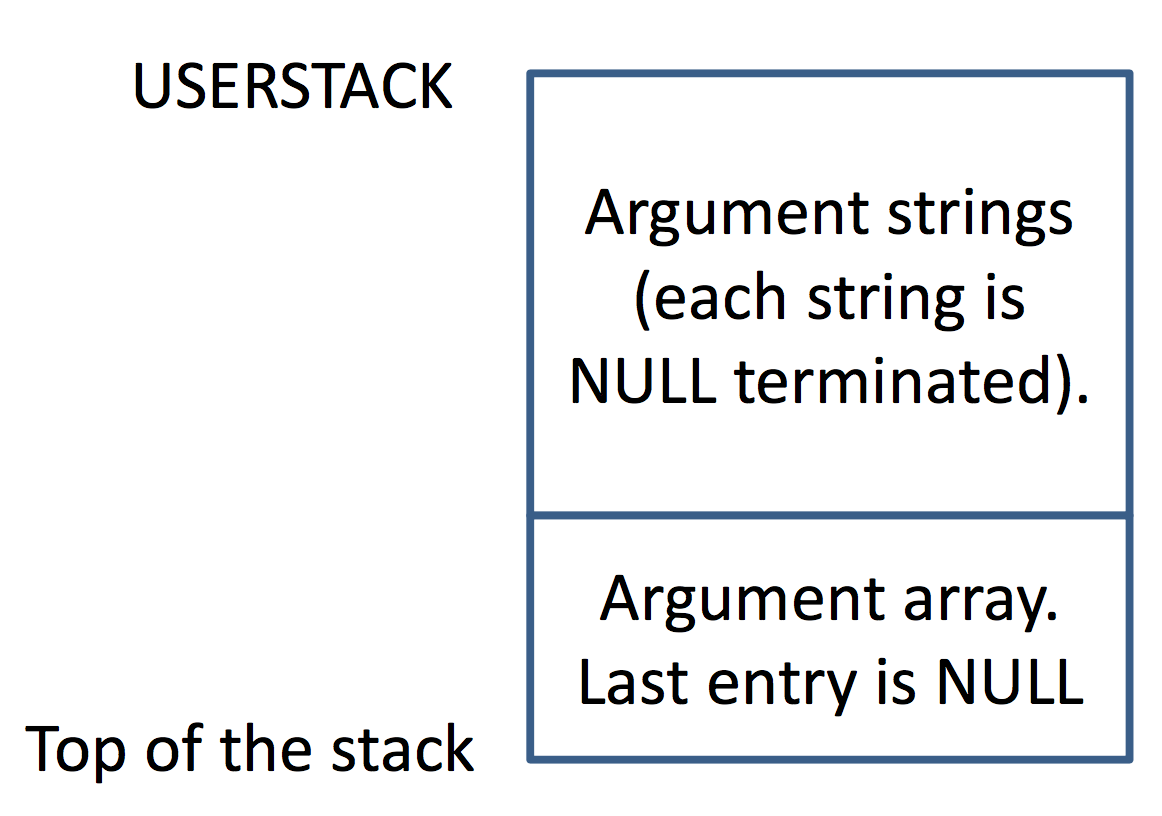
\includegraphics[scale=0.3]{pictures/2b_alignment.png}
  \end{center}
\end{wrapfigure}
When storing items on the stack, pad each item such that they are 8-byte aligned. \\
e.g., \texttt{args\_size = ROUNDUP(args\_size, 8);} \\

Strings don't have to be 4 or 8-byte aligned. However, pointers to strings need to be 4-byte aligned.


%%%%%%%%%%%%%%%%%%%n
%% VIRTUAL MEMORY %%
%%%%%%%%%%%%%%%%%%%%
\newpage
\section{Virtual Memory}
\subsection{Physical Memory and Addresses}
\begin{figure}[H]
  \centering
  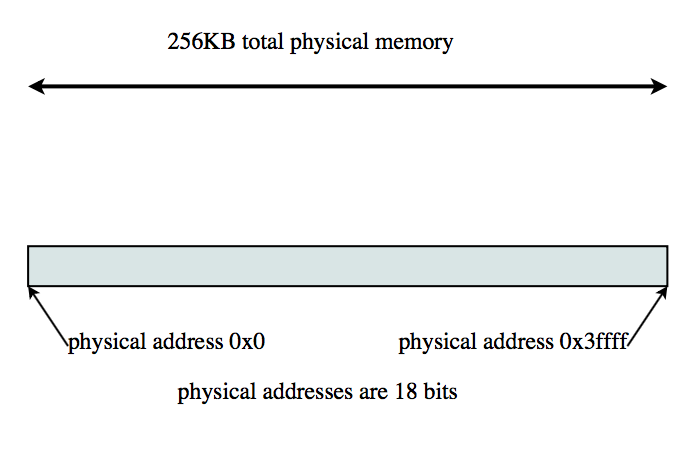
\includegraphics[scale=0.65]{pictures/phys_mem.png}
  \caption{An example physical memory, $P = 18$}
  \label{fig:phys_mem}
\end{figure}
If physical addresses have $P$ \emph{bits}, the maximum amount of addressable physical memory is $2^{P}$ \emph{bytes} (assuming a byte-addressable machine).
\begin{itemize}
  \item Sys/161 MIPS processor uses 32 bit physical addresses ($P = 32$) $\Rightarrow$ maximum physical memory size of $2^{32}$ bytes, or 4GB
  \item Larger values of $P$ are common on modern processors, e.g., $P = 48$, which allows 256TB of physical memory to be addressed
\end{itemize}

The actual amount of physical memory on a machine may be less than the maximum amount that can be addressed.

\subsection{Virtual Memory and Addresses}
\begin{figure}[H]
  \centering
  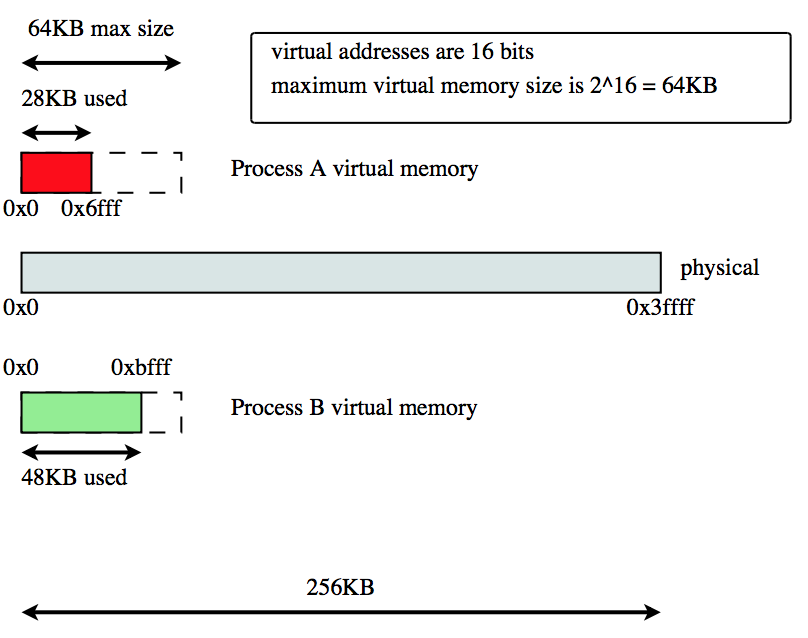
\includegraphics[scale=0.65]{pictures/v_mem.png}
  \caption{An example of virtual memory, $V = 16$}
  \label{fig:v_mem}
\end{figure}
The kernel provides a separate, private \emph{virtual} memory for each process. \\
The virtual memory of a process holds the code, data, and stack for the program that is running in that process. \\
If virtual addresses are $V$ bits, the \emph{maximum} size of a virtual memory is $2^{V}$ bytes.
\begin{itemize}
  \item For the MIPS, $V = 32$
\end{itemize}
Running applications see only virtual addresses, e.g.,
\begin{itemize}
  \item program counter and stack pointer hold \emph{virtual addresses} of the next instruction and the stack
  \item pointers to variables are \emph{virtual addresses}
  \item jumps/branches refer to \emph{virtual addresses}
\end{itemize}
Each process is isolated in its virtual memory, and cannot access other process' virtual memories.

\subsection{Address Translation}
Each virtual memory is mapped to a different part of physical memory. \\
Since virtual memory is not real, when an process tries to access (load or store) a virtual address, the virtual address is \emph{translated} (mapped) to its corresponding physical address, and the load or store is performed in physical memory. \\
Address translation is performed in hardware, using information provided by the kernel.

\subsection{Address Translation for Dynamic Relocation}
\begin{figure}[H]
  \centering
  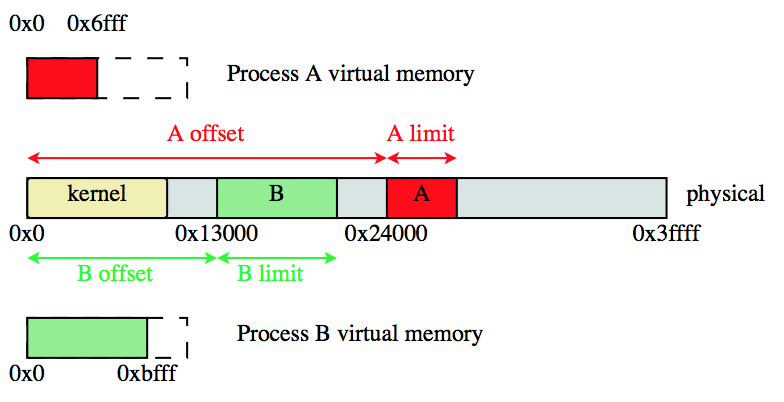
\includegraphics[scale=0.6]{pictures/dyn_reloc.png}
  \caption{Example of dynamic relocation}
  \label{fig:dyn_reloc_ex}
\end{figure}
CPU includes a \emph{memory management unit} (MMU), with a \emph{relocation register} and a \emph{limit register}.
\begin{itemize}
  \item relocation register holds the physical offset ($R$) for the running process' virtual memory
  \item limit register holds the size $L$ of the running process' virtual memory
\end{itemize}
To translate a virtual address $v$ to a physical address $p$:
\begin{align*}
&\texttt{if } v \geq L \texttt{ then generate exception} \\
&\texttt{else} \\
&\qquad p \leftarrow v + R
\end{align*}
Translation is done in hardware by the MMU. \\
The kernel maintains a separate $R$ and $L$ for each process, and changes the values in the MMU registers when there is a context switch between processes. \\

\begin{ex*}
$v = \texttt{0x102c} \qquad p = \texttt{0x102c} + \texttt{0x24000} = \texttt{0x2502c}$ \\
$v = \texttt{0x8800} \qquad p = \texttt{exception}$ since $\texttt{0x8800} \geq \texttt{0x7000}$
\end{ex*}

\subsection{Properties of Dynamic Relocation}
Each virtual address space corresponds to a \emph{contiguous range of physical addresses}. \\
The kernel is responsible for deciding \emph{where} each virtual address space should map in physical memory.
\begin{itemize}
  \item the OS must track which part of physical memory are in use, and which parts are free
  \item since different address spaces may have different sizes, the OS must allocate/deallocate variable-sized chunks of physical memory
  \item hence creates potential for \emph{fragmentation} of physical memory
\end{itemize}

\subsection{Paging}
\subsubsection{Paging: Physical Memory}
Physical memory is divided into fixed-size chunks called \emph{frames} or \emph{physical pages}.
\begin{figure}[H]
  \centering
  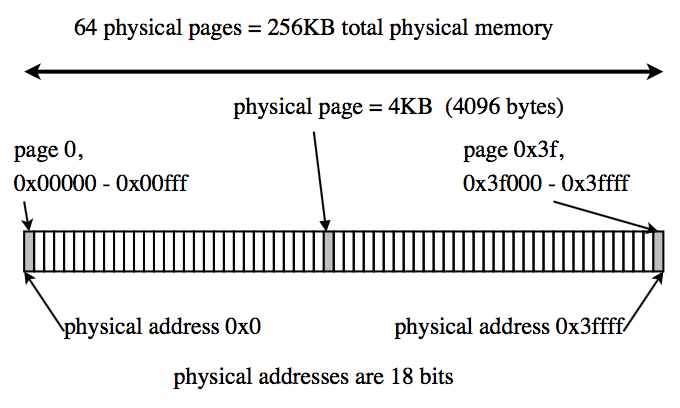
\includegraphics[scale=0.7]{pictures/paging_phys_mem.png}
  \caption{The frame size if $2^{12}$ bytes (4KB)}
  \label{fig:p_phys_mem}
\end{figure}

\subsubsection{Paging: Virtual Memory}
Virtual memories are divided into fixed-size chunks called \emph{pages}. \\
Page size is equal to frame size.
\begin{figure}[H]
  \centering
  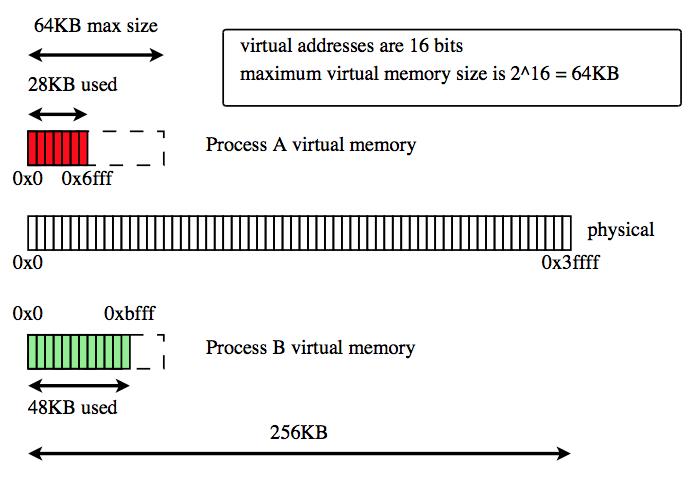
\includegraphics[scale=0.8]{pictures/paging_v_mem.png}
  \caption{Page size is 4KB here}
  \label{fig:p_v_mem}
\end{figure}

\subsubsection{Paging: Address Translation}
\begin{figure}[H]
  \centering
  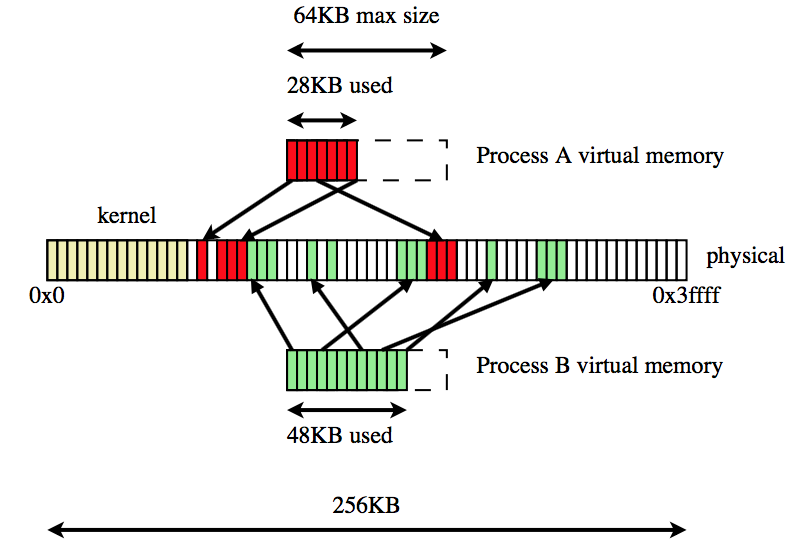
\includegraphics[scale=0.7]{pictures/p_translation.png}
  \label{fig:p_trans}
\end{figure}
Each page maps to a different frame.
Any page can map to any frame.

\subsubsection{Paging: Address Translation}
The MMU includes a \emph{page table base register} which points to the page table for the current process. \\

How the MMU translate a virtual address:
\begin{enumerate}
  \item[1.] determines the \emph{page number} and \emph{offset} of the virtual address
  \begin{itemize}
    \item page number is the virtual address divided by the page size
    \item offset is the virtual address modulo the page size
  \end{itemize}
  \item[2.] looks up the page's entry (PTE) in the current process page table, using the page number
  \item[3.] if the PTE is not valid, raise an exception
  \item[4.] otherwise, combine page's frame number from the PTE with the offset to determine the physical address;
  physical address is $(\text{frame number} \cdot \text{frame size}) + \text{offset}$ \\
\end{enumerate}

\subsubsection{Other Information Found in PTEs}
PTEs may contain other fields, in addition to the frame number and valid bit. \\

Example 1: write protection bit
\begin{itemize}
  \item can be set by the kernel to indicate that a page is read-only
  \item if a write operation (e.g., MIPS \texttt{lw}) uses a virtual address on a read-only page, the MMU will raise an exception when it translate the virtual address
\end{itemize}

Example 2: bits to track page usage
\begin{itemize}
  \item reference (use) bit: has the process used this page recently?
  \item dirty bit: have contents of this page been changed?
  \item these bits are set by the MMU, and read by the kernel
\end{itemize}

\subsubsection{Page Tables: How Big?}
A page table has one PTE for each page in the virtual memory
\begin{itemize}
  \item $\text{page table size} = \text{number of pages} \cdot \text{size of PTE}$
  \item $\text{number of pages} = \frac{\text{virtual memory size}}{\text{page size}}$
\end{itemize}
The page table of a 64KB virtual memory, with 4KB pages, is 64 bytes, assuming 32 \emph{bits} for each PTE. \\
Page tables for larger virtual memories are larger.

\subsubsection{Page Tables: Where?}
Page tables are kernel data structures, i.e. page tables for all processes are in the kernel's stack.

\subsection{Summary: Roles of the Kernel and the MMU}
Kernel:
\begin{itemize}
  \item Manage MMU (memory management unit) registers on address space switches (context switch from thread in one process to thread in a different process)
  \item Create and manage page tables
  \item Manage (allocate/deallocate) physical memory
  \item Handle exceptions raised by the MMU
\end{itemize}
Memory Management Unit, MMU, (hardware):
\begin{itemize}
  \item Translate virtual addresses to physical addresses
  \item Check for and raise exceptions when necessary
\end{itemize}

\subsection{TLBs}
Execution of each machine instruction may involve one, two, or more memory operations
\begin{itemize}
  \item one to fetch instruction
  \item one or more for instruction operands
\end{itemize}
Address translation through a page table adds one extra memory operation (for page table entry lookup) for each memory operation performed during instruction execution. \\
This can be slow! \\

Solution: include a \emph{Translation Lookaside Buffer} (TLB) in the MMU,
\begin{itemize}
  \item TLB is a small, fast, dedicated cache for address translation in the MMU
  \item Each TLB entry stores a (page number $\Rightarrow$ frame number) mapping
\end{itemize}

\subsubsection{TLB Use}
What the MMU does to translate a virtual address on page $p$:
\begin{verbatim}
  if there is an entry (p, f) in the TLB then
    return f  /* TLB hit! */
  else
    find p's frame number (f) from the page table
    add (p, f) to the TLB, evicting another entry if full
    return f  /* TLB miss */
\end{verbatim}
If the MMU cannot distinguish TLB entries from different address spaces, then the kernel must \emph{clear} or \emph{invalidate} the TLB on \emph{each} context switch from one process to another! \\

This is a \emph{hardware-managed TLB},
\begin{itemize}
  \item the MMU handles TLB misses, including page table lookup and replacement of TLB entries
  \item MMU must understand the kernel's page table format
\end{itemize}

\subsubsection{Software-Managed TLBs}
The MIPS has a \emph{software-managed TLB}, which translates a virtual address on page $p$ like this:
\begin{verbatim}
  if there is an entry (p,f) in the TLB then
    return f        /* TLB hit! */
  else
    raise exception /* TLB miss */
\end{verbatim}
In case of a TLB miss, the kernel must
\begin{enumerate}
  \item[1.] determine the frame number of $p$
  \item[2.] add $(p, f)$ to the TLB, evicting another entry if necessary
\end{enumerate}
After the miss is handled, the instruction that caused the exception is re-tried.

\begin{figure}[H]
  \centering
  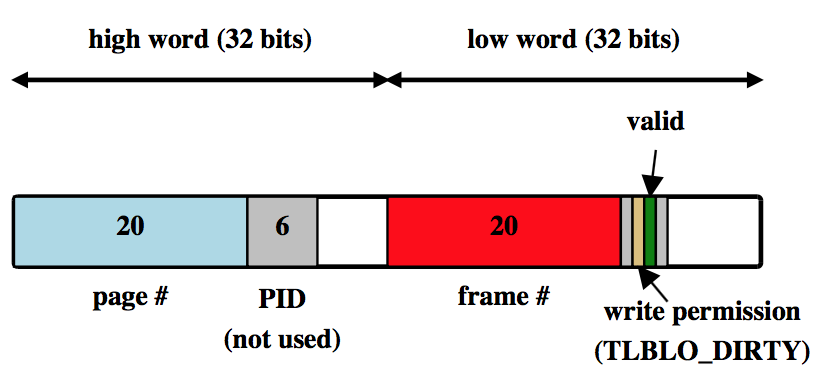
\includegraphics[scale=0.6]{pictures/mips_tlb.png}
  \caption{The MIPS R3000 TLB}
  \label{fig:mips_tlb}
\end{figure}
The MIPS TLB has room for 64 entries. Each entry is 64 bits (8 bytes) long.

\subsection{Large, Sparse Virtual Memories}
\begin{figure}[H]
  \centering
  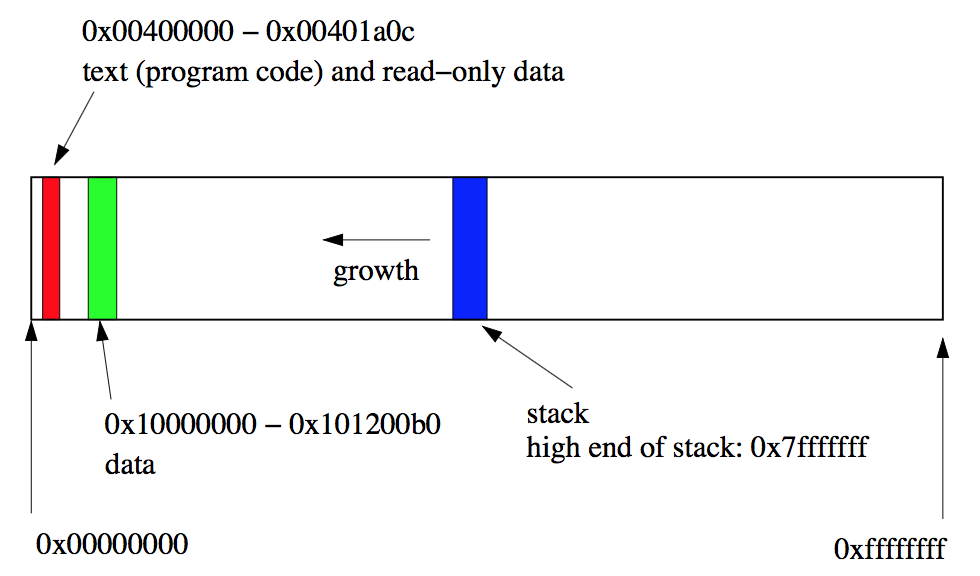
\includegraphics[scale=0.65]{pictures/real_v_mem.png}
  \caption{A more realistic virtual memory; this is a layout of the virtual address space for \texttt{user/testbin/sort} in OS/161}
  \label{fig:realistic_v_mem}
\end{figure}
Virtual memory may be large,
\begin{itemize}
  \item[MIPS:] $V = 32$, max virtual memory is $2^{32}$ bytes (4 GB)
  \item[x86-64:] $V = 48$, max virtual memory is $2^{48}$ bytes (256 TB)
\end{itemize}
Much of the virtual memory may be unused (see \ref{fig:realistic_v_mem})! \\

Application may use \emph{discontinuous segments} of the virtual memory. \\
One reason is that we have to give room for the stack to grow in the virtual memory!

\subsection{Limitations of Simple Address Translation Approaches}
A kernel that used simple dynamic relocation would have to allocate 2 GB of contiguous physical memory for \texttt{testbin/sort}'s virtual memory, even though \texttt{sort} only uses about 1.2 MB. \\

A kernel that used simple paging would require a page table with $2^{20}$ PTEs (assuming page size is 4 KB) to map \texttt{testbin/sort}'s address space,
\begin{itemize}
  \item this page table is actually larger than the virtual memory that \texttt{sort} needs to use
  \item most of the PTEs are marked as invalid
  \item this page table has to be contiguous in kernel memory
\end{itemize}

\subsection{Segmentation}
\begin{figure}[H]
  \centering
  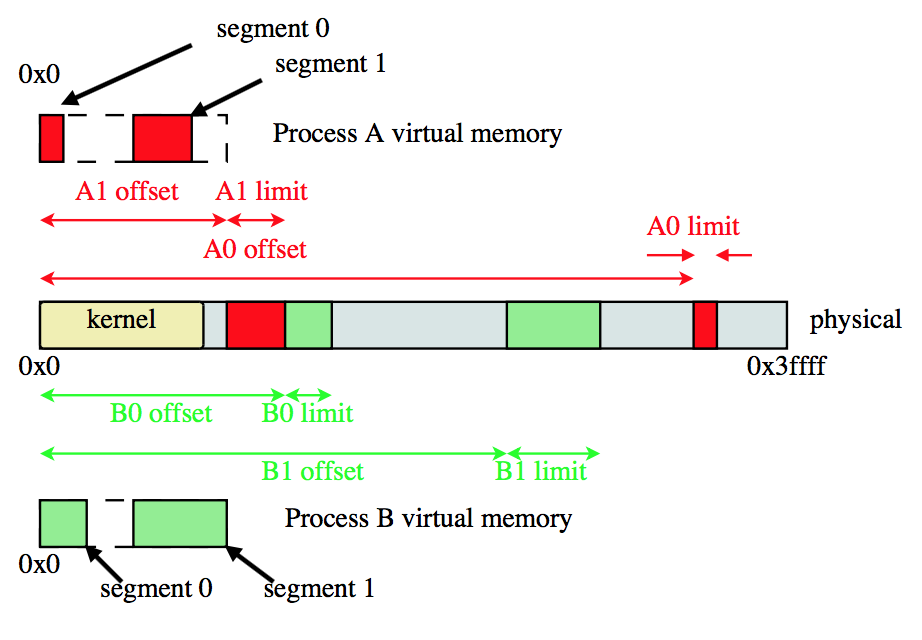
\includegraphics[scale=0.65]{pictures/seg_addr_space.png}
  \caption{Example of segment address space}
  \label{fig:seg_addr_space}
\end{figure}
Instead of mapping the entire virtual memory to physical, we can provide a separate mapping for each segment of the virtual memory that the application actually uses. \\

Instead of a single offset and limit for the entire address space, the kernel maintains an offset and limit for each segment,
\begin{itemize}
  \item The MMU has multiple offset and limit registers, one pair for each segment
\end{itemize}

With segmentation, a virtual address can be thought of as having two parts: segment ID and offset within segment. \\

With $K$ bits for the segment ID, we can have up to:
\begin{itemize}
  \item $2^{K}$ segments
  \item $2^{V - K}$ bytes per segment
\end{itemize}

The kernel decides where each segment is placed in physical memory.
Fragmentation of physical memory is possible!

\subsection{Translating Segmented Virtual Addresses}
The MMU needs a relocation register and a limit register for each segment,
\begin{itemize}
  \item let $R_{i}$ be the relocation offset for the $i$th segment
  \item let $L_{i}$ be the limit of the $i$th segment
\end{itemize}
To translate virtual address $v$ to a physical address $p$:
\begin{align*}
&\texttt{split } p \texttt{ into segment number }(s)\texttt{ and address within segment }(a) \\
&\texttt{if } a \geq L_{s} \texttt{ then generate exception} \\
&\texttt{else} \\
&\quad p \gets a + R_{s}
\end{align*}
As for dynamic relocation, the kernel maintains a separate set of relocation offsets and limits for each process, and changes the values in the MMU's registers when there is a context switch between processes.

\subsection{Two-Level Paging}
Instead of having a single page table to map an entire virtual memory, we can split the page table into smaller page tables, and add page table directory.
\begin{itemize}
  \item Instead of one larger, contiguous table, we have multiple smaller tables
  \item If all PTEs in a small table are invalid, we can avoid creating that table entirely
\end{itemize}
\begin{figure}[H]
  \centering
  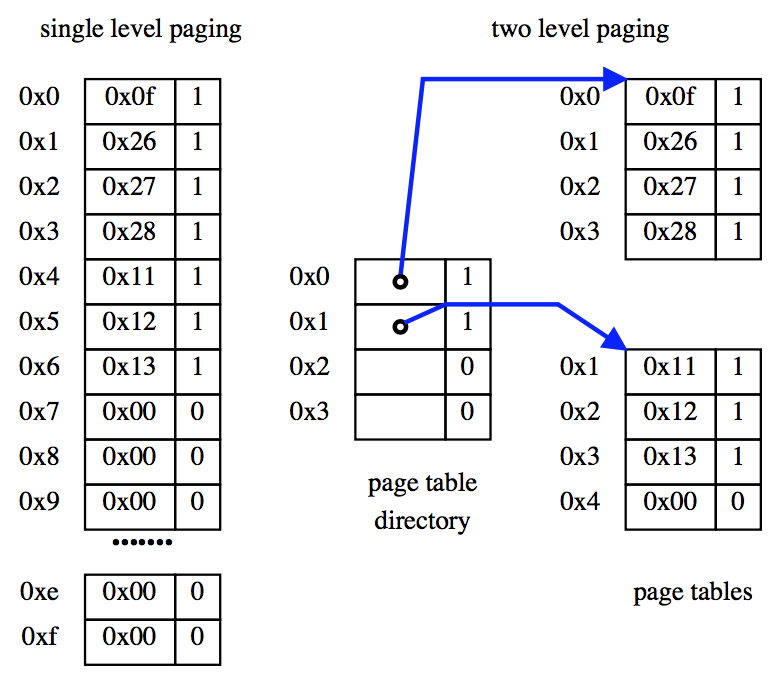
\includegraphics[scale=0.7]{pictures/single_double_paging.png}
  \caption{Single vs. Two Level Paging}
  \label{fig:s_t_paging}
\end{figure}
Each virtual address has three parts:
\begin{enumerate}
  \item[1.] Level one page number: used to index the directory
  \item[2.] Level two page number: used to index a page table
  \item[3.] Offset within the page
\end{enumerate}

\subsection{Address Translation with Two-Level Paging}
\begin{figure}[H]
  \centering
  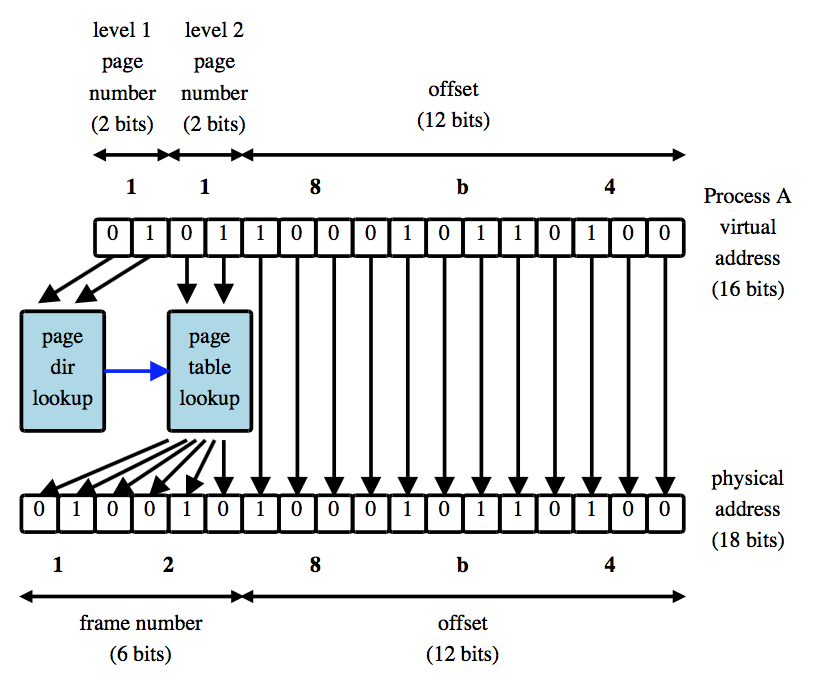
\includegraphics[scale=0.7]{pictures/two_level_paing_trans.png}
  \caption{Example of two-level address translation}
  \label{fig:two_level_addr_translation}
\end{figure}
The MMU's \emph{page table base register} points to the page table directory for the current process. \\
Each virtual address $v$ has three parts: $(p_{1}, p_{2}, o)$ \\
How the MMU translate a virtual address:
\begin{enumerate}
  \item[1.] Index into the page table directory using $p_{1}$ to get a pointer to a 2nd level page table
  \item[2.] If the directory entry is not valid, raise an exception
  \item[3.] Index into the 2nd level page table using $p_{2}$ to find the PTE for the page being accessed
  \item[4.] If the PTE is not valid, raise an exception
  \item[5.] Otherwise, combine the frame number from the PTE with $o$ to determine the physical address (as for single-level paging)
\end{enumerate}

\subsection{Limits of Two-Level Paging}
A goal of two-level paging was to keep individual page tables small. \\
Suppose we have 40 bit virtual addresses ($V = 40$) and that
\begin{itemize}
  \item the size of a PTE is 4 bytes
  \item page size is 4KB ($2^{12}$ bytes)
  \item we'd like to limit each page table's size to 4KB
\end{itemize}
Problem: for large address spaces, we may need a large page table directory!
\begin{itemize}
  \item There can be up to $2^{28}$ pages in a virtual memory
  \item A single page table can hold $2^{10}$ PTEs
  \item We may need up to $2^{18}$ page tables
  \item Our page table directory will have to have $2^{18}$ entries
  \item If a directory entry is 4 bytes, the directory will occupy 1MB
\end{itemize}
This is the problem we were trying to avoid by introducing a second level!

\subsection{Multi-Level Paging}
We can solve the large directory problem by introducing additional levels of directories. \\
Example: 4-level paging in x86-64 architecture. \\
Properties of Multi-Level Paging:
\begin{itemize}
  \item can map large virtual memories by adding more levels
  \item individual page table/directories can remain small
  \item can avoid allocating page tables and directories that are not needed for programs that use a small amount of virtual memory
  \item TLB misses become \emph{more} expensive as the number of levels goes up, since more directories must be accessed to find the correct PTE
\end{itemize}

\subsection{Virtual Memory in OS/161 on MIPS: \texttt{dumbvm}}
The MIPS uses 32-bit paged virtual and physical addresses. \\
The MIPS has a software-managed TLB,
\begin{itemize}
  \item TLB raises an exception on every TLB miss
  \item kernel is free to record page-to-frame mappings however it wants to
\end{itemize}

TLB exceptions are handled by a kernel function called \texttt{vm\_fault} \\
\texttt{vm\_fault} uses information from an \texttt{addrspace} structure to determine a page-to-frame mapping to load into the TLB,
\begin{itemize}
  \item there is a separate \texttt{addrspace} structure for each process
  \item each \texttt{addrspace} structure describes where its process's pages are stored in physical memory
  \item an \texttt{addrspace} structure does the same job as a page table, but the \texttt{addrspace} structure is simpler because OS/161 places all pages of each segment \emph{contiguously} in physical memory
\end{itemize}

\subsubsection{The \texttt{addrspace} Structure}
\begin{figure}[H]
  \centering
  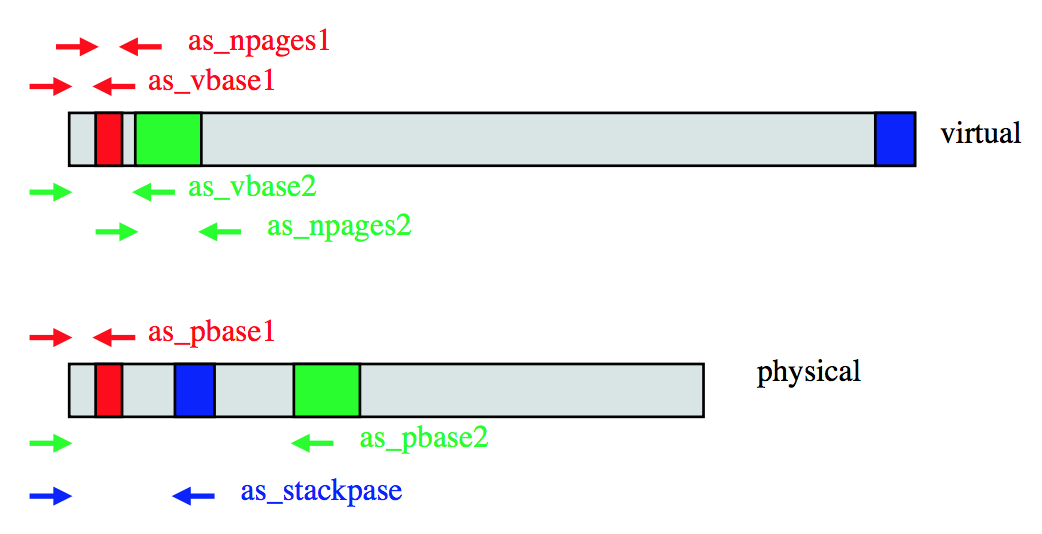
\includegraphics[scale=0.7]{pictures/addrspace.png}
  \caption{\texttt{addrspace} diagram}
  \label{fig:addrspace}
\end{figure}
\begin{verbatim}
  struct addrspace {
    vaddr_t as_vbase1;      /* base virtual address of code segment */
    paddr_t as_pbase1;      /* base physical address of code segment */
    size_t as_npages1;      /* size (in pages) of code segment */
    vaddr_t as_vbase2;      /* base virtual address of data segment */
    paddr_t as_pbase2;      /* base physical address of data segment */
    size_t as_npages2;      /* size (in pages) of data segment */
    paddr_t as_stackpbase;  /* base physical address of stack */
  };
\end{verbatim}

\subsubsection{Address Translation: OS/161 dumbvm Example}
\textbf{Note}: in OS/161, the stack is 12 pages and the page size is 4 KB = 0x1000. \\
\begin{table}[H]
  \vspace{-20pt}
  \centering
  \begin{tabular}{|r|r|r|}
  \hline
  Variable/Field & Process 1 & Process 2 \\ \hline \hline
  as\_vbase1 & 0x0040 0000 & 0x0040 0000 \\ \hline
  as\_pbase1 & 0x0020 0000 & 0x0050 0000 \\ \hline
  as\_bpages1 & 0x0000 0008 & 0x0000 0002 \\ \hline
  as\_vbase2 & 0x1000 0000 & 0x1000 0000 \\ \hline
  as\_pbase2 & 0x0080 0000 & 0x00A0 0000 \\ \hline
  as\_npages & 0x0000 0010 & 0x0000 0008 \\ \hline
  as\_stackpbase & 0x0010 0000 & 0x00B0 0000 \\ \hline
  \end{tabular}
\end{table}

\subsection{Initializing an Address Space}
When the kernel creates a process to run a particular program, it must create an address space for the process, and load the program's code and data into that address space. \\
OS/161 \emph{pre-loads} the address space before the program runs.
Many other OS load pages on \emph{demand}. \\

A program's code and data is described in an \emph{executable file}, which is created when the program is compiled and linked. \\

OS/161 (and some other operating systems) expect executable files to be in ELF (\textbf{E}xecutable and \textbf{L}inking \textbf{F}ormat) format. \\

The OS/161 execv system call re-initializes the address space of a process
\begin{verbatim}
  int execv (const char* program, char** args)
\end{verbatim}

The \texttt{program} parameter of the \texttt{execv} system call should be the name of the ELF executable file for the program that is to be loaded into the address space.

\subsection{ELF Files}
ELF files contain address space segment descriptions, which are useful to the kernel when it is loading a new address space. \\

The ELF file identifies the (virtual) address of the program's first instruction. \\

The ELF file also contains lots of other information (e.g., section descriptors, symbol tables) that is useful to compilers, linkers, debuggers, loaders, and other tools used to build programs.

\subsubsection{Address Space Segments in ELF Files}
The ELF file contains a header describing the segments and segment \emph{images}. \\

Each ELF segment describes a contiguous region of the virtual address space. \\

The header includes an entry for each segment which describes:
\begin{itemize}
  \item the virtual address of the start of the segment
  \item length of the segment in the virtual address space
  \item location of the start of the segment image in the ELF file (if present)
  \item the length of the segment image in the LEF file (if present)
\end{itemize}

The image is an exact copy of the binary data that should be loaded into specified portion of the virtual address space. \\

The image may be smaller than the address space segment, in which case the rest of the address space segment is expected to be zero-filled. \\

In OS/161, the kernel copies segment images from the ELF file to the specified portions of the virtual address space.

\subsubsection{ELF Files and OS/161}
\begin{figure}[H]
  \centering
  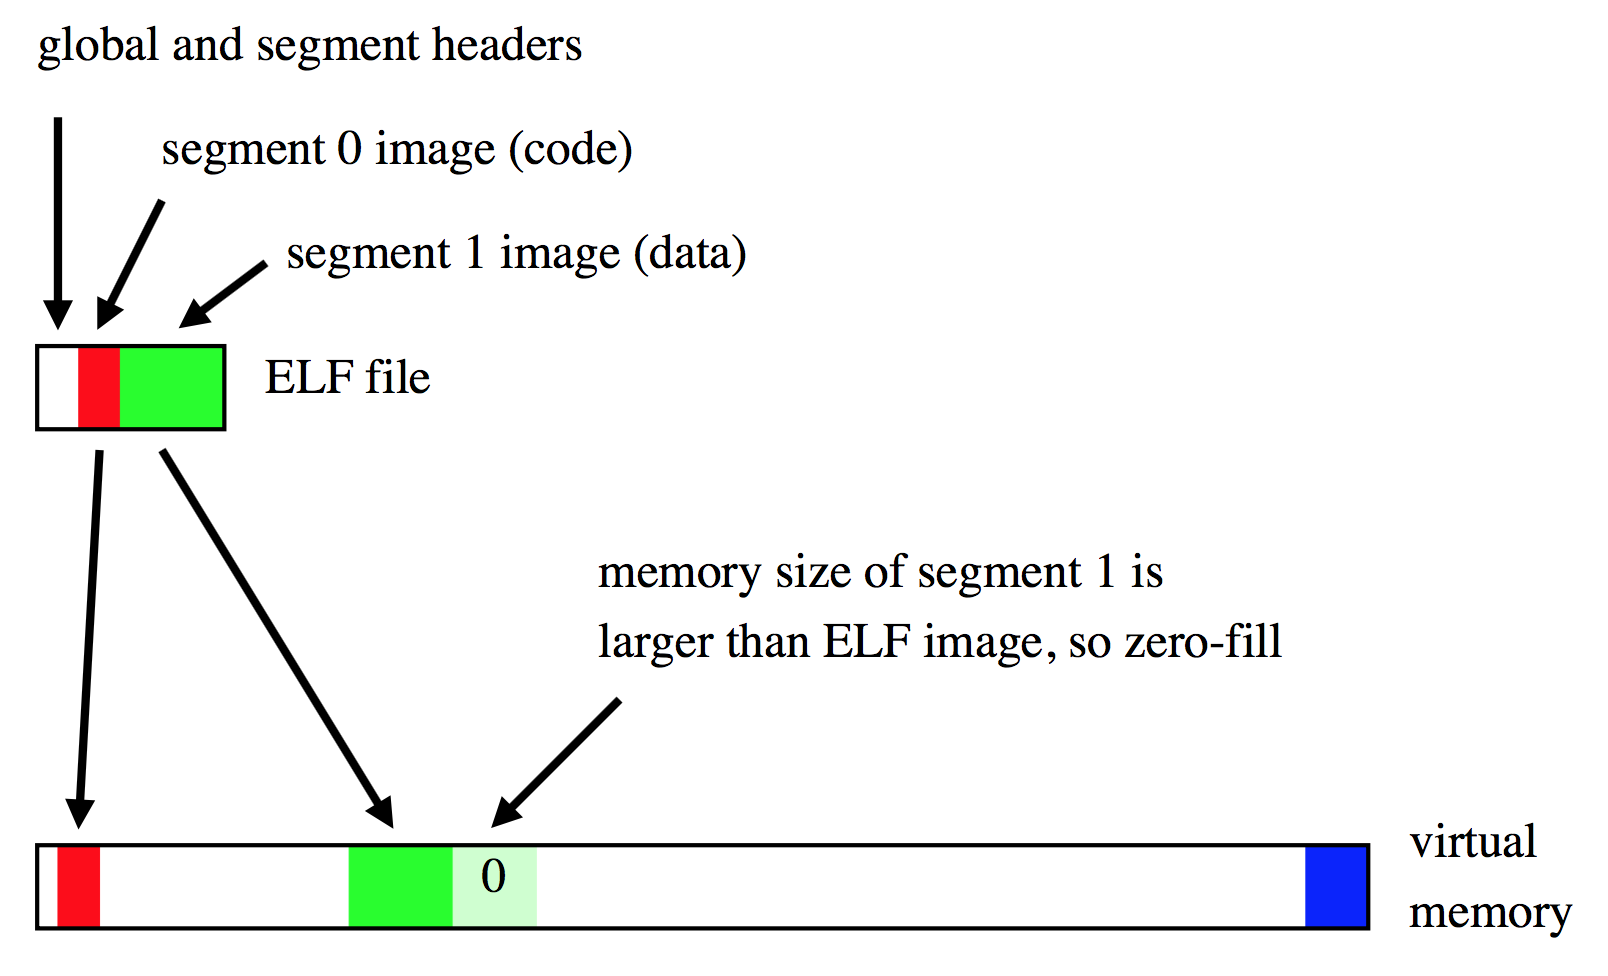
\includegraphics[scale=0.39]{pictures/elf_diagram.png}
  \caption{ELF File Diagram}
  \label{fig:elf}
\end{figure}
OS/161's \texttt{dumbvm} implementation assumes that an LEF file contains two segments:
\begin{itemize}
  \item a \emph{text segment}, containing the program code and any read-only data
  \item a \emph{data segment}, containing any other global program data
\end{itemize}

The ELF file does \emph{not} describe the stack. \\

\texttt{dumbvm} creates a \emph{stack segment} for each process.
It is 12 pages long, ending at virtual address \texttt{0x7fffffff}.


\subsection{Virtual Memory for the Kernel}
We would like the kernel to live in virtual memory, but there are some challenges:
\begin{itemize}
  \item[\textbf{Bootstrapping}:] since the kernel helps to implement virtual memory, how can the kernel run in virtual memory when it is just starting?
  \item[\textbf{Sharing}:] sometimes data need to be copied between the kernel and application programs?
  How can this happen if they are in different virtual address spaces?
\end{itemize}

\begin{figure}[H]
  \centering
  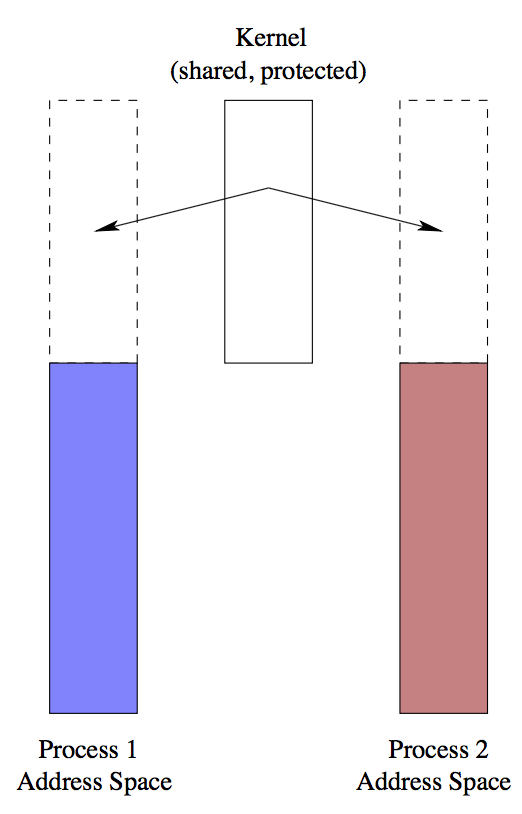
\includegraphics[scale=0.55]{pictures/kernel_v_mem.png}
  \caption{The Kernel in Process' Address Spaces}
  \label{fig:kernel_v_mem}
\end{figure}

The sharing problem can be addressed by making the kernel's virtual memory \emph{overlap} with process' virtual memories. \\
Attempts to access kernel code/data is user mode results in memory protection exceptions, not invalid address exception. \\

Solutions to the bootstrapping problem are architecture-specific.

\begin{figure}[H]
  \centering
  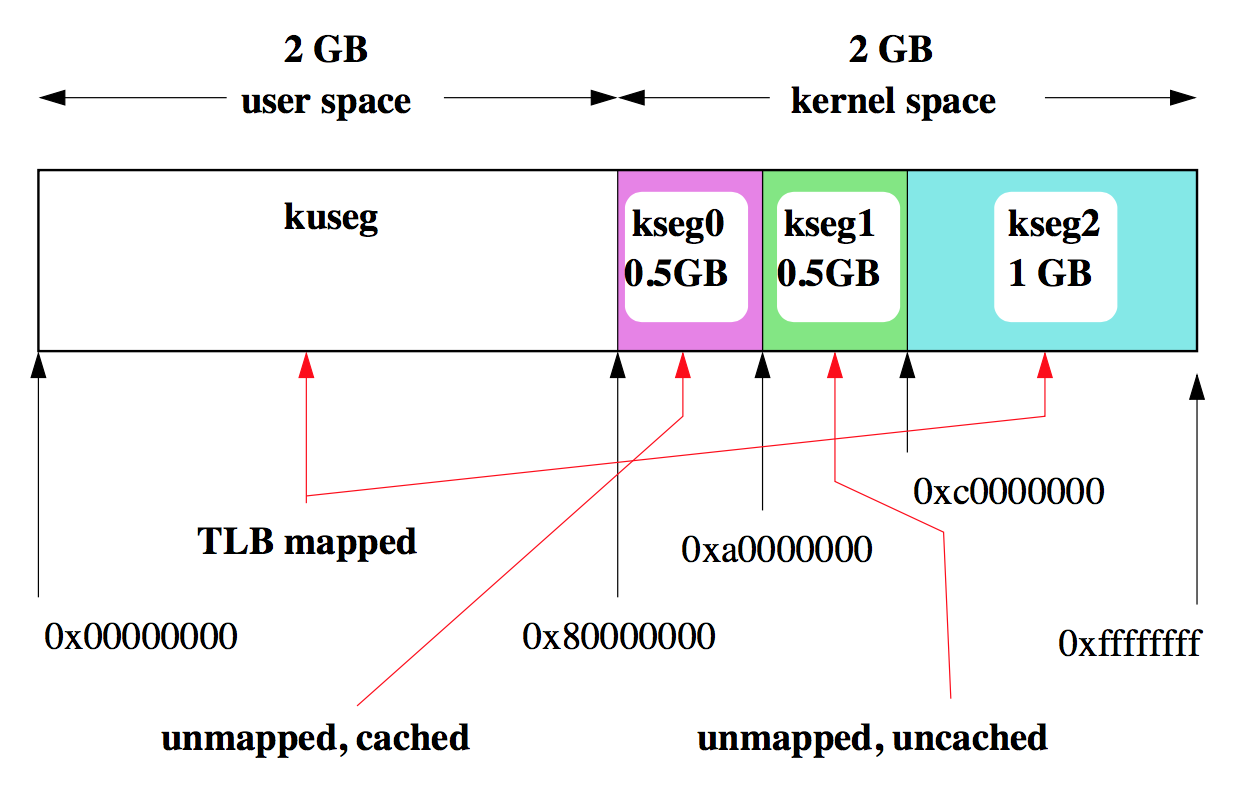
\includegraphics[scale=0.5]{pictures/user_kernel_space_mips.png}
  \caption{User Space and Kernel Space on the MIPS R3000}
  \label{fig:mips_space}
\end{figure}

In OS/161, user programs live in kuseg, kernel code and data structures live in kseg0, devices are accessed through kseg1, and kseg2 is not used.

\subsection{Exploiting Secondary Storage}
\textbf{Goals}:
\begin{itemize}
  \item Allow virtual address spaces that are larger than the physical address space
  \item Allow greater multiprogramming levels by using less of the available (primary) memory for each process
\end{itemize}

\textbf{Method}:
\begin{itemize}
  \item Allow pages from virtual memories to be stored in secondary storage, i.e., on disks or SSDs
  \item Swap pages (or segments) between secondary storage and primary storage so that they are in primary memory when needed
\end{itemize}

\subsection{Resident Sets and Present Bits}
When swapping is used, some pages of each virtual memory will be in memory, and others will not be in memory.
\begin{itemize}
  \item The set of virtual pages present in physical memory is called the \emph{resident set} of a process.
  \item A process's resident set will change over time as pages are swapped in and out of physical memory
\end{itemize}

To track which pages are in physical memory, each PTE needs to contain an extra bit, called the present bit:
\begin{itemize}
  \item valid = 1, present = 1: page is valid and in memory
  \item valid = 1, present = 0: page is valid, but not in memory
  \item value = 0, present - $x$: invalid page
\end{itemize}

\subsection{Page Faults}
When a process tries to access a page that is not in memory, the problem is detected because the page's \emph{present} bit is zero:
\begin{itemize}
  \item on a machine with a hardware-managed TLB, the MMU detects this when it checks the page's PTE, and generates an exception, which the kernel must handle
  \item on a machine with a software-managed TLB, the kernel detects the problem when it checks the page's PTE after a TLB miss
\end{itemize}

This event (attempting to access a non-resident page) is called a \emph{page fault}. \\

When a page fault happens, it is the kernel's job to:
\begin{enumerate}
  \item[1.] swap the page into memory from secondary storage, evicting another page from memory if necessary
  \item[2.] update the PTE (set the \emph{present} bit)
  \item[3.] return from the exception so that the application can retry the virtual memory access that caused the page fault
\end{enumerate}

\subsection{Secondary Storage is Slow}
Access times for disks are measured in \emph{milli}seconds, SSD read latencies are 10’s-100’s of \emph{micro}seconds. \\

Both of these are much higher than memory access times (100’s of \emph{nano}seconds) \\

Suppose that secondary storage access is 1000 times slower than memory access.
Then:
\begin{itemize}
  \item if there is one page fault every 10 memory accesses (on average), the average memory access time with swapping will be about 100 times larger than it would be without swapping
  \item if there is one page fault every 100 memory accesses (on average), the average memory access time with swapping will be about 10 times larger than it would be without swapping
  \item if there is one page fault every 1000 memory accesses (on average), the average memory access time with swapping will be about 2 times larger than it would be without swapping.
\end{itemize}

\subsection{Performance with Swapping}
To provide good performance for virtual memory accesses, the kernel should try to ensure that page faults are rare. \\

Some techniques the kernel can use to improve performance:
\begin{itemize}
  \item limit the number of processes, so that there is enough physical memory per process
  \item try to be smart about \emph{which} pages are kept in physical memory, and which are evicted
  \item hide latencies, e.g., by \emph{prefetching} pages before a process needs them
\end{itemize}

\subsubsection{A Simple Replacement Policy: FIFO}
Replace the page that has been in memory the longest.
\begin{table}[H]
  \vspace{-20pt}
  \caption{Three-frame example}
  \centering
  \begin{tabular}{|r|c|c|c|c|c|c|c|c|c|c|c|c|}
  \hline
  Num & 1 & 2 & 3 & 4 & 5 & 6 & 7 & 8 & 9 & 10 & 11 & 12 \\ \hline
  Refs & a & b & c & d & a & b & e & a & b & c & d & e \\ \hline
  \hline
  Frame 1 & a & a & a & d & d & d & e & e & e & e & e & e \\ \hline
  Frame 2 &  & b & b & b & a & a & a & a & a & c & c & c \\ \hline
  Frame 3 &  &  & c & c & c & b & b & b & b & b & d & d \\ \hline
  Fault ? & x & x & x & x & x & x & x &  &  & x & x &  \\ \hline
  \end{tabular}
\end{table}

\subsubsection{Optimal Page Replacement}
MIN: replace the page that will not be referenced for the longest time. \\
MIN requires knowledge of the future.

\begin{table}[H]
  \vspace{-20pt}
  \caption{Three-frame example}
  \centering
  \begin{tabular}{|r|c|c|c|c|c|c|c|c|c|c|c|c|}
  \hline
  Num & 1 & 2 & 3 & 4 & 5 & 6 & 7 & 8 & 9 & 10 & 11 & 12 \\ \hline
  Refs & a & b & c & d & a & b & e & a & b & c & d & e \\ \hline
  \hline
  Frame 1 & a & a & a & a & a & a & a & a & a & c & c & c \\ \hline
  Frame 2 &  & b & b & b & b & b & b & b & b & b & d & d \\ \hline
  Frame 3 &  &  & c & d & d & d & e & e & e & e & e & e \\ \hline
  Fault ? & x & x & x & x &  &  & x &  &  & x & x &  \\ \hline
  \end{tabular}
\end{table}

\subsubsection{Least Recently Used (LRU) Page Replacement}
\begin{table}[H]
  \vspace{-20pt}
  \caption{Three-frame example}
  \centering
  \begin{tabular}{|r|c|c|c|c|c|c|c|c|c|c|c|c|}
  \hline
  Num & 1 & 2 & 3 & 4 & 5 & 6 & 7 & 8 & 9 & 10 & 11 & 12 \\ \hline
  Refs & a & b & c & d & a & b & e & a & b & c & d & e \\ \hline
  \hline
  Frame 1 & a & a & a & d & d & d & e & e & e & c & c & c \\ \hline
  Frame 2 &  & b & b & b & a & a & a & a & a & a & d & d \\ \hline
  Frame 3 &  &  & c & c & c & b & b & b & b & b & b & e \\ \hline
  Fault ? & x & x & x & x & x & x & x &  &  & x & x & x \\ \hline
  \end{tabular}
\end{table}

\subsection{Locality}
Real programs do not access their virtual memories randomly. \\
Instead, they exhibit \emph{locality}:
\begin{itemize}
  \item \textbf{temporal locality}: programs are more likely to access pages that they have accessed recently than pages that they have not accessed recently
  \item \textbf{spatial locality}: programs are likely to access parts of memory that are close to parts of memory they have accessed recently
\end{itemize}

Locality helps the kernel keep page fault rates low.

\subsection{Measuring Memory Accesses}
The kernel is not aware which pages a program is using unless there is an exception. \\
This makes it difficult for the kernel to exploit locality by implementing a replace policy like LRU. \\

The MMU can help solve this program by tracking page accesses in hardware. \\
Simple scheme: add a \emph{use bit} (or \emph{reference bit}) to each PTE.
This bit:
\begin{itemize}
  \item is set by the MMU each time the page is used, i.e., each time the MMU translates a virtual address on that page
  \item can be read and cleared by the kernel
\end{itemize}

The use bit provides a small amount of memory usage information that can be exploited by the kernel.

\subsection{The Clock Replacement Algorithm}
The clock algorithm (also known as ``second chance'') is one of the simplest algorithms that exploits the use bit. \\

Clock is identical to FIFO, except that a page is ``skipped'' if its use bit is set. \\

The clock algorithm can be visualized as a victim pointer that cycles through the page frames. \\
The pointer moves whenever a replacement is necessary:
\begin{verbatim}
  while use bit of victim is set
    clear use bit of victim
    victim = (victim + 1) % num_frames
  choose victim for replacement
  victim = (victim + 1) % num_frames
\end{verbatim}


%%%%%%%%%%%%%%%%
%% SCHEDULING %%
%%%%%%%%%%%%%%%%
\newpage
\section{Scheduling}
\subsection{Simple Scheduling Model}
We are given a set of \emph{jobs} to schedule. \\
Only one job can run at a time. \\
For each job, we are given
\begin{itemize}
  \item job arrival time ($a_{i}$)
  \item job run time ($r_{i}$)
\end{itemize}
For each job, we define
\begin{itemize}
  \item \emph{response time}: time between the job's arrival and when the job starts to run
  \item \emph{turnaround time}: time between the job's arrival and when the job finishes running
\end{itemize}
We must decide when each job should run, to achieve some goal, e.g., minimize average turnaround time, or minimize average response time.

\subsection{Basic Non-Preemptive Schedulers: FCFS and SJF}
\emph{FCFS}: run jobs in arrival time order.
\begin{itemize}
  \item simple, avoids starvation
  \item pre-emptive variant: round-robin
\end{itemize}

\emph{SFJ}: shortest job first --- run jobs in increasing order of $r_{i}$
\begin{itemize}
  \item minimizes average \emph{turnaround} time
  \item long jobs may starve
  \item pre-emptive variant: SRTF (shortest remaining time first)
\end{itemize}

\subsection{CPU Scheduling}
In CPU scheduling, the ``jobs'' to be scheduled are the threads. \\
CPU scheduling typically differs from the simple scheduling model:
\begin{itemize}
  \item the run times of threads are normally not known
  \item threads are sometimes not runnable: when they are blocked
  \item threads may have different priorities
\end{itemize}

The objective of the scheduler is normally to achieve a balance between
\begin{itemize}
  \item responsiveness (ensure that threads get to run regularly)
  \item fairness
  \item efficiency
\end{itemize}

\subsection{Multi-level Feedback Queues}
Objective: good responsiveness for \emph{interactive} threads, non-interactive threads make as much progress as possible. \\
Key idea: interactive threads are frequently blocked. \\
Approach: given higher priority to interactive threads, so that they run whenever they are ready. \\
Problem: how to determine which threads are interactive and which are not? \\

\textbf{Algorithm} \\
Scheduler maintains $n$ round-robin ready queues $(Q_{1}, \dots, Q_{n})$. \\
Scheduler always chooses a thread from $Q_{n}$, unless it is empty
\begin{itemize}
  \item if $Q_{n}$ is empty, choose a thread from $Q_{n - 1}$, unless it is empty too
  \item and so on, choosing a thread from $Q_{1}$ only if all other queues are empty.
\end{itemize}
Threads in queue $Q_{i}$ uses quantum $q_{i}$, typically larger quanta for lower-priority threads ($q_{i} \geq q_{i + 1}$). \\
If the running thread from $Q_{i}$ uses its entire quantum and gets preempted, demote it to queue $Q_{i - 1}$. \\
If a thread blocks, put it into $Q_{n}$ when it wakes up. \\
To prevent starvation, periodically move all threads to $Q_{n}$.

\begin{figure}[H]
  \centering
  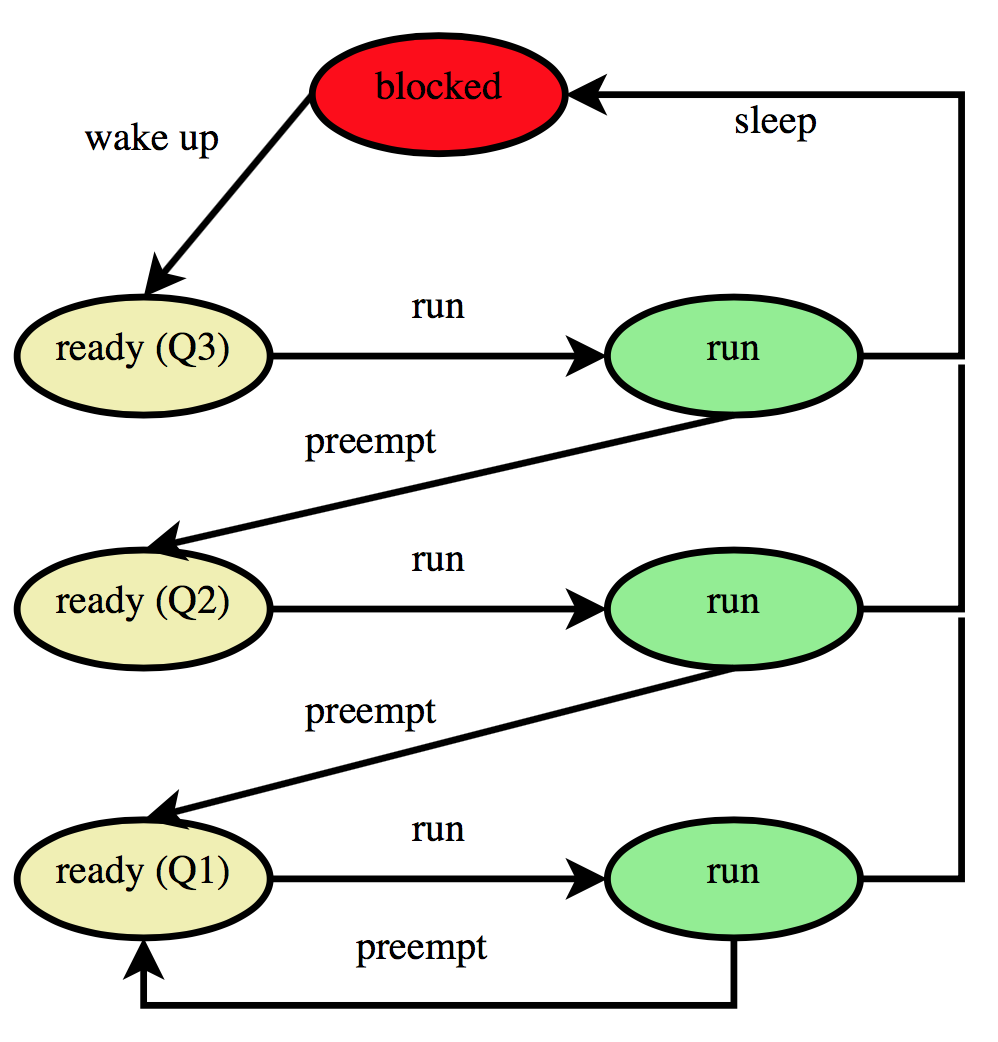
\includegraphics[scale=0.5]{pictures/3-level_queue.png}
  \caption{3 Level Feedback Queue State Diagram}
  \label{fig:3levelfeedback}
\end{figure}

\subsection{Linux Complexity Fair Scheduler (CFS) - Main Ideas}
Each thread can be assigned a \emph{weight}. \\
The goal of the scheduler is to ensure that each thread gets a ``share'' of the processor in proportion to its weight. \\

Basic operation:
\begin{itemize}
  \item track the ``virtual'' run time of each run-able thread
  \item always run the thread with the lowest virtual run time
\end{itemize}

Virtual run time is actual run time adjusted by the thread weights
\begin{itemize}
  \item suppose $w_{i}$ is the weight of the $i$th thread
  \item actual run time of $i$th thread is multiplied by $\frac{\sum_{j}w_{j}}{w_{i}}$
  \item virtual run time advances slowly for threads with high weights, quickly for threads with low weights
\end{itemize}

\subsection{Scheduling on Multi-Core Processors}
\begin{figure}[H]
  \centering
  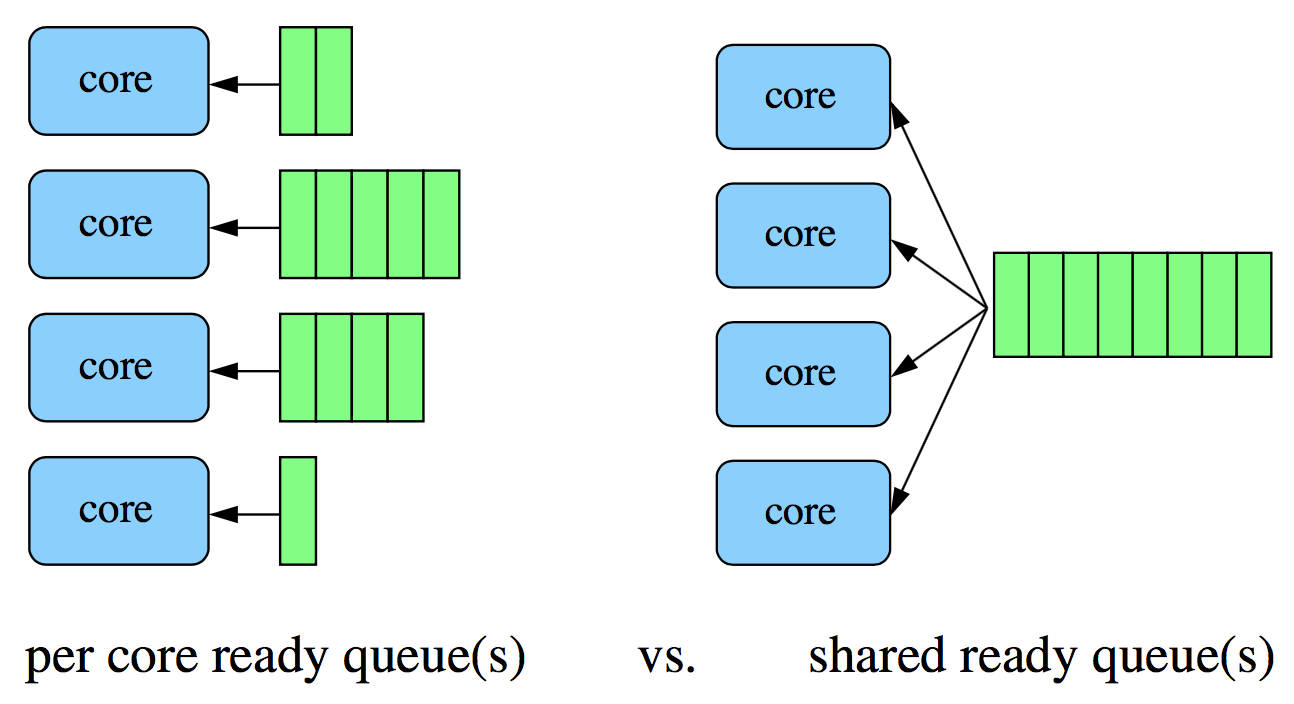
\includegraphics[scale=0.5]{pictures/multicore_scheduling.png}
\end{figure}

\subsubsection{Scalability and Cache Affinity}
Contention and Scalability
\begin{itemize}
  \item access to shared ready queue is a critical section, mutual exclusion needed
  \item as number of cores grows, contention for ready queue becomes a problem
  \item per core design \emph{scales} to a larger number of cores
\end{itemize}

CPU cache affinity
\begin{itemize}
  \item as thread runs, data it accesses is loaded into CPU cache(s)
  \item moving the thread to another core means data must be reloaded into that core's caches
  \item as thread runs, it acquires an \emph{affinity} for one core because of the cached data
  \item per core design benefits from affinity by keeping threads on the same core
  \item shared queue design does not
\end{itemize}

\subsubsection{Load Balancing}
In per-core design, queues may have different lengths. \\
This results in \emph{load imbalance} across the cores,
\begin{itemize}
  \item cores may be idle while others are busy
  \item threads on lightly loaded cores get more CPU time than threads on heavily loaded cores
\end{itemize}

Not an issue in shared queue design. \\

Per-core designs typically need some mechanism for \emph{thread migration} to address load imbalances,
\begin{itemize}
  \item migration means moving threads from heavily loaded cores to lightly loaded cores
\end{itemize}

%%%%%%%%%%%%%%%%%%%%%%%%%
%% ASSIGNMENT 3 REVIEW %%
%%%%%%%%%%%%%%%%%%%%%%%%%
\newpage
\section{Assignment 3 Review}
\texttt{dumbvm} is a very limited virtual memory system,
\begin{itemize}
  \item A full TLB leads to a kernel panic
  \item Text segment is not read-only
  \item Uses fixed segmentation (external fragmentation)
  \item Never reuses physical memory (required restarting the OS after each test)
\end{itemize}

\subsection{TLB Replacement}
VM related exceptions are handled by \texttt{vm\_fault} \\

\texttt{vm\_fault} performs address translation and loads the virtual address to physical address mapping into the TLB.
\begin{itemize}
  \item Iterates through the TLB to find an unused/invalid entry
  \item Overwrites the unused entry with the virtual to physical address mapping required by the instruction that generated the TLB exception
\end{itemize}

If the TLB is full, call \texttt{tlb\_random} to write the entry into a random TLB slot,
\begin{itemize}
  \item that's it for TLB replacement!
  \item make sure that virtual page fields in the TLB are unique.
\end{itemize}

\subsection{Read-Only Text Segment}
Currently, TLB entries are loaded with \texttt{TLBLO\_DIRTY} on.
\begin{itemize}
  \item Pages are therefore read and writable.
\end{itemize}

Text segment should be read-only.
\begin{itemize}
  \item Load TLB entries for the text segment with \texttt{TLBLO\_DIRTY} off.
  \item \texttt{elo \&= \textasciitilde TLBLO\_DIRTY;}
\end{itemize}

Determine the segment of the fault address by looking at the \texttt{vbase} and \texttt{vtop} addresses. \\

Unfortunately, this will cause \texttt{load\_elf} to throw a \texttt{VM\_FAULT\_READONLY} exception.
\begin{itemize}
  \item It is trying to write to a memory location that is read-only.
\end{itemize}

We must instead load TLB entries with \texttt{TLBLO\_DIRTY} on until \texttt{load\_elf} has completed.
\begin{itemize}
  \item Consider adding a flag to \texttt{struct addrspace} to indicate whether or not \texttt{load\_elf} has completed.
  \item When \texttt{load\_elf} completes, flush the TLB, and ensure that all future TLB entries for the text segment has \texttt{TLBLO\_DIRTY} off.
\end{itemize}

Writing to read-only memory address will lead to a \texttt{VM\_FAULT\_READONLY} exception. \\
This will currently cause a kernel panic. \\

Instead of panicking, your VM system should kill the process. \\
Modify \texttt{kill\_curthread} to kill the current thread,
\begin{itemize}
  \item very similar to \texttt{sys\_\_exit}.
  However, the exit code/status will be different.
  \item Consider which signal number this will trigger (look at the beginning of \texttt{kill\_curthread}).
\end{itemize}

\subsection{Managing Memory}
During bootstrap, the kernel allocates memory by calling \texttt{getppages}, which in turn calls \texttt{ram\_stealmem(pages)}. \\

\texttt{ram\_stealmem} just allocates pages without providing any mechanism to release pages (see \texttt{free\_kpages}). \\

We want to manage our own memory after bootstrap. \\

In \texttt{vm\_bootstrap}, call \texttt{ram\_getsize} to get the remaining physical memory in the system. \\
Do \emph{not} call \texttt{ram\_stealmem} again! \\

Logically partition the memory into fixed size frames. \\
Each frame is \texttt{PAGE\_SIZE} bytes. \\

Keep track of the status of each frame (core-map data structure). \\

Where should we store the core-map data structure? \\
Store it in the start of the memory return by \texttt{ram\_getsize}. \\
The frames should start after the core-map data structure. \\
The core-map should track which frames are used and available. \\
It should also keep track of contiguous memory allocations, because frames need to be contiguous.

\subsection{Alloc and Free}
\texttt{alloc\_kpages(int npages)}:
\begin{itemize}
  \item Allocate frames for both \texttt{kmalloc} and address spaces
  \item Frames need to be contiguous
\end{itemize}

\texttt{kfree\_kpages(vaddr\_t addr)}:
\begin{itemize}
  \item Free pages allocated with \texttt{alloc\_kpages}
  \item We don't specify how many pages we need to free.
  It should free the same number of pages that was allocated.
  \item Update core-map to make frames available after \texttt{free\_kpages}
\end{itemize}

Consider adding some information in the core-map to help determine the number of pages that need to be free. \\
e.g. If 4 contiguous frames were allocated using \texttt{alloc\_kpages}, then store 4 in the core-map entry for the start for the start of the four frames.

\subsection{Page Tables}
In order to avoid external fragmentation, we need to introduce paging. \\
New VM system combines segmentation with page. \\
Three segments:
\begin{itemize}
  \item Text (read-only)
  \item Data
  \item Stack
\end{itemize}
Create a page table for each segment,
\begin{itemize}
  \item each page table entry should include the frame number
\end{itemize}

In \texttt{dumbmvm}, \texttt{struct addrspace} has the following fields:
\begin{itemize}
  \item \texttt{vaddr\_t as\_vbase1}
  \item \texttt{paddr\_t as\_pbase1}
  \item \texttt{size\_t as\_npages1}

  \item \texttt{vaddr\_t as\_vbase2}
  \item \texttt{paddr\_t as\_pbase2}
  \item \texttt{size\_t as\_npages2}

  \item \texttt{paddr\_t as\_stackpbase}
\end{itemize}

With segmentation and paging, replace \texttt{pbase} with page table. \\

\texttt{as\_create}:
\begin{itemize}
  \item Initialize address space data structures
\end{itemize}

\texttt{as\_define\_region}:
\begin{itemize}
  \item A region is essentially a segment
  \item Allocate (\texttt{kmalloc}) and initialize the page table for the specified segment
  \item Size of the segment is a parameter of \texttt{as\_define\_region}
  \begin{itemize}
    \item Because we perform preloading, segment size will never grow
    \item Size of the page table is based on the segment size
  \end{itemize}
  \item Setup the read/write permissions for this segment
  \item Optionally have permissions per page
\end{itemize}

\texttt{as\_prepare\_load}:
\begin{itemize}
  \item Pre-allocate frames for each page in the segment
  \item Frames do not need to be contiguous
  \item Allocate each frame one at a time
\end{itemize}

\texttt{as\_define\_stack}:
\begin{itemize}
  \item Always allocate \texttt{NUM\_STACK\_PAGES} for the stack
  \item Need to create a page table for the stack
  \item Need to allocate frames for the stack
  \begin{itemize}
    \item \texttt{as\_prepare\_load} only allocates frames for segments that were defined by \texttt{load\_elf}
    \item Stack segment is not defined by \texttt{load\_elf}
  \end{itemize}
\end{itemize}

\texttt{as\_copy}:
\begin{itemize}
  \item Call \texttt{as\_create} to create the address space
  \item Create segments based on old address space
  \item Allocate frames for the segments
  \item \texttt{memcpy} frames from the old address space to the frames in the new address space
\end{itemize}

\texttt{as\_destroy}:
\begin{itemize}
  \item Call \texttt{free\_kpages} on the frames for each segment
  \item \texttt{kfree} the page tables
\end{itemize}

\subsection{User Address/Kernel Virtual Address/Physical Address}
Remember that you are always working with virtual addresses,
\begin{itemize}
  \item only use physical addresses when loading entries in the TLB.
  \item virtual addresses are converted either by the TLB or by the MMU directly.
\end{itemize}

Addresses below 0x8000 0000 are user space addresses that are TLB mapped. \\

Addresses between 0x8000 0000 and 0xa000 0000 are kernel virtual addresses that are converted by the MMU directly, $\text{kernel virtual address} - 0\text{x}8000~0000 = \text{physical address}$. \\

\texttt{kmalloc} always return a kernel virtual address. \\
Do \emph{not} use \texttt{kmalloc} to allocate frames.

%%%%%%%%%%%%%%%%%%%%%
%% DEVICES AND I/O %%
%%%%%%%%%%%%%%%%%%%%%
\newpage
\section{Devices and I/O}
\subsection{Sys/161 Device Examples}
\begin{itemize}
  \item timer/clock --- current time, timer, beep
  \item disk drive --- persistent storage
  \item serial console --- character input/output
  \item text screen --- character-oriented graphics
  \item network interface --- packet input/output
\end{itemize}

\begin{table}[H]
  \vspace{-20pt}
  \caption{Sys/161 timer/clock}
  \label{tab:sys161_timer}
  \centering

  \begin{tabular}{|c|c|c|l|}
  \hline
  Offset & Size & Type & Description \\ \hline \hline
  0 & 4 & status & current time (seconds) \\ \hline
  4 & 4 & status & current time (nanoseconds) \\ \hline
  8 & 4 & command & restart-on-expiry \\ \hline
  12 & 4 & status and command & interrupt (reading clears) \\ \hline
  16 & 4 & status and command & countdown time (microseconds) \\ \hline
  20 & 4 & command & speaker (cause beeps) \\ \hline
  \end{tabular}
\end{table}

\begin{table}[H]
  \vspace{-20pt}
  \caption{Serial Console}
  \label{tab:serial_con}
  \centering

  \begin{tabular}{|c|c|c|l|}
  \hline
  Offset & Size & Type & Description \\ \hline \hline
  0 & 4 & command and data & character buffer \\ \hline
  4 & 4 & status & writeIRQ \\ \hline
  8 & 4 & status & readIRQ \\ \hline
  \end{tabular}
\end{table}

\subsection{Device Drivers}
A device driver is a part of the kernel that interacts with a device.

\begin{ex*}
Write character to serial output device.
\begin{verbatim}
  // only one writer at a time
  P(output device write semaphore)
  // trigger the write operation
  write character to device data register
  repeat {
    read writeIRQ register
  } until status is "complete"
  // make the device ready again
  write writeIRQ register to acknowledge completion
  V(output device write semaphore)
\end{verbatim}
This illustrates \emph{polling}: the kernel driver repeatedly checks device status
\end{ex*}

\subsubsection{Using Interrupts to Avoid Polling}
\textbf{Device Driver Write Handler}:
\begin{verbatim}
  // only one writer at a time
  P(output device write semaphore)
  // trigger write operation
  write character to device data register
\end{verbatim}
\medskip
\textbf{Interrupt Handler for Serial Device}:
\begin{verbatim}
  // make the device ready again
  write writeIRQ register to acknowledge completion
  V(output device write semaphore)
\end{verbatim}

\subsubsection{Accessing Devices}
\textbf{Option 1}: special I/O instructions
\begin{itemize}
  \item such as \texttt{in} and \texttt{out} instructions on x86
  \item device registers are assigned ``port'' numbers
  \item instructions transfer data between a specified port and a CPU register
\end{itemize}
\medskip
\textbf{Option 2}: memory-mapped I/O
\begin{itemize}
  \item each device register has a physical memory address
  \item device drivers can read from or write to device registers using normal load and store instructions, as though accessing memory
\end{itemize}

\subsection{MIPS/OS161 Physical Address Space}
\begin{figure}[H]
  \centering
  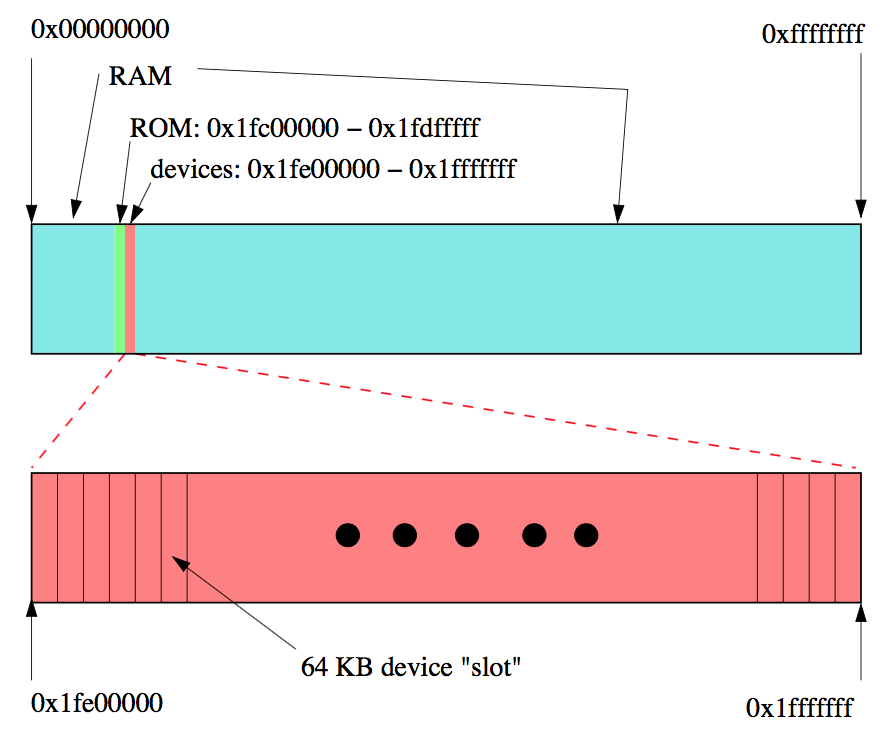
\includegraphics[scale=0.55]{pictures/os161_addrspace.png}
  \caption{Each device is assigned to one of 32 64KB device ``slots''. A device's registers and data buffers are memory-mapped into its assigned slot.}
  \label{fig:os161_addrspace}
\end{figure}

\subsection{Logical View of a Disk Drive}
Disk is an array of of numbered blocks (or sectors). \\
Each block is the same size (e.g. 512 bytes). \\

Blocks are the unit of transfer between the disk and memory. \\
Typically, one or more contiguous blocks can be transferred in a single operation. \\

Storage is \emph{non-volatile}, i.e., data persists even when the device is without power.

\begin{figure}[H]
  \centering
  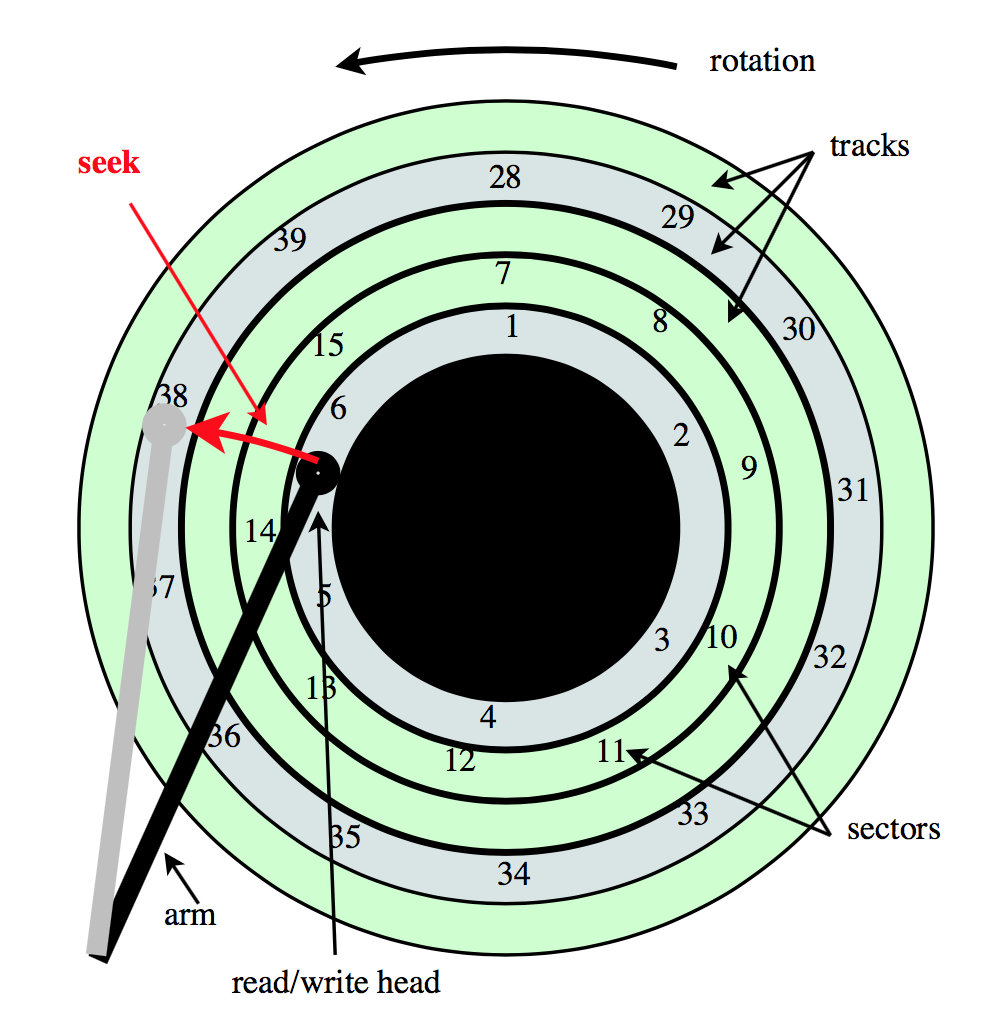
\includegraphics[scale=0.4]{pictures/disk_platter.png}
  \caption{A disk platter's surface}
  \label{fig:disk_platter}
\end{figure}

\subsubsection{Cost Model for Disk I/O}
Moving data to/from a disk involves:
\begin{itemize}
  \item \textbf{seek time}: move the read/write heads to the appropriate cylinder.
  Depends on the distance (in tracks) between previous request and current request --- called the \emph{seek distance}.

  \item \textbf{rotational latency}: wait until the desired sectors spin to the read/write heads.
  Depends on the rotational speed of the disk.

  \item \textbf{transfer time}: wait while the desired sectors spin past the read/write heads.
  Depends on the rotational speed of the disk and the amount of data being read/written.
\end{itemize}

Request service time is the \emph{sum} of seek time, rotational latency, and transfer time.

\subsubsection{Seek, Rotation, and Transfer}
Seek Time:
\begin{itemize}
  \item If the next request is for data on the same track as the previous request, seek distance and seek time will be zero.
  \item In the worst case, e.g., seek from outermost track to innermost track, seek time may be 10 milliseconds or more.
\end{itemize}
\medskip
Rotational Latency:
\begin{itemize}
  \item Consider a disk that spins at $12,000$ RPM.
  \item One complete rotation takes 5 milliseconds.
  \item Rotational latency ranges from 0ms to 5ms.
\end{itemize}
\medskip
Transfer Time:
\begin{itemize}
  \item Once positioned, the $12,000$ RPM disk can read/write all data on a track in one rotation (5ms).
  \item If only $x\%$ of the track's sectors are being read/written, transfer time will be $x\%$ of the complete rotation time (5ms).
\end{itemize}

\subsubsection{Performance Implications of Disk Characteristics}
Larger transfers to/from a disk device are \emph{more efficient} than smaller ones. \\
That is, the cost (time) per byte is smaller for larger transfers. \\

Sequential I/O is faster than non-sequential I/O. \\
Sequential I/O operations eliminate the need for (most) seeks.

\subsection{Disk Head Scheduling}
Goal: reduce seek times by controlling the order in which requests are serviced. \\

Disk head scheduling may be performed by the device, by the operating system, or both. \\

For disk head scheduling to be effective, there must be a queue of outstanding disk requests (otherwise there is nothing to reorder). \\

An on-line approach is required: new I/O requests may arrive at any time.

\subsubsection{FCFS Disk Head Scheduling}
\begin{figure}[H]
  \centering
  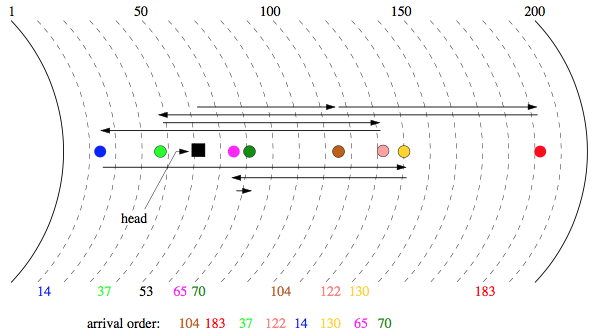
\includegraphics[scale=0.5]{pictures/fcfs_disk.png}
\end{figure}
Handle requests in the order in which they arrive. \\
Fair and simple, but no optimization of seek times.

\subsubsection{Shortest Seek Time First (SSTF)}
\begin{figure}[H]
  \centering
  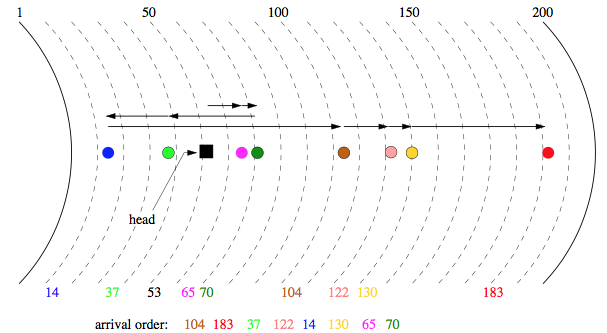
\includegraphics[scale=0.5]{pictures/sstf_disk.png}
\end{figure}
Choose closest request (a greedy approach). \\
Seek times are reduced, but requests may starve.

\subsubsection{Elevator Algorithms (SCAN)}
\begin{figure}[H]
  \centering
  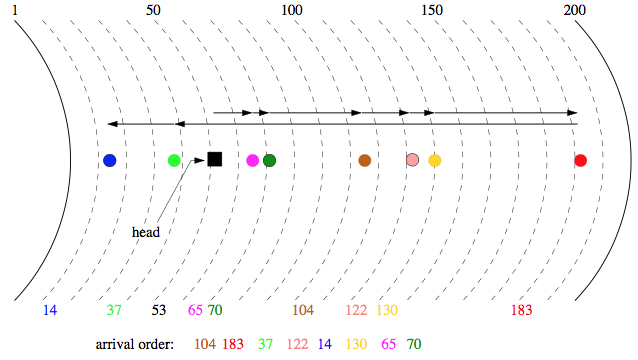
\includegraphics[scale=0.5]{pictures/scan_disk.png}
\end{figure}
Under SCAN, aka the elevator algorithm, the disk head moves in one direction until there are no more requests in front of it, then reverses direction. \\
There are many variations on this idea. \\

SCAN reduces seek times (relative to FCFS), while avoiding starvation.

\subsection{Data Transfer To/From Devices}
Option 1: \emph{program-controlled I/O} \\
The device driver moves the data between memory and a buffer on the device.
\begin{itemize}
  \item Simple, but the CPU is \emph{busy} while the data is being transferred.
\end{itemize}
\medskip
Option 2: \emph{direct memory access} (DMA)
\begin{itemize}
  \item The device itself is responsible for moving data to/from memory.
  CPU is \emph{not busy} during this data transfer, and is free to do something else.
\end{itemize}

Sys/161 disks do program-controlled I/O.
\begin{table}[H]
  \vspace{-20pt}
  \caption{Sys/161 Disk Controller}
  \label{tab:sys1161_disk_control}
  \centering

  \begin{tabular}{|c|c|c|l|}
  \hline
  Offset & Size & Type & Description \\ \hline \hline
  0 & 4 & status & number of sectors \\ \hline
  4 & 4 & status and command & status \\ \hline
  8 & 4 & command & sector number \\ \hline
  12 & 4 & status & rotational speed (RPM) \\ \hline
  32768 & 512 & data & transfer buffer \\ \hline
  \end{tabular}
\end{table}

\subsubsection{Writing to a Sys/161 Disk}
\textbf{Device Driver Write Handler}
\begin{verbatim}
  // only one disk request at a time
  P(disk semaphore)
  copy data from memory to device transfer buffer
  write target sector number to disk sector number register
  write "write" command to disk status register
  // wait for request to complete
  P(disk completion semaphore)
  V(disk semaphore)
\end{verbatim}
\medskip
\textbf{Interrupt Handler for Disk Device}
\begin{verbatim}
  // make the device ready again
  write disk status register to acknowledge completion
  V(disk completion semaphore)
\end{verbatim}

\subsubsection{Reading from a Sys/161 Disk}
\textbf{Device Driver Read Handler}
\begin{verbatim}
  // only one disk request at a time
  P(disk semaphore)
  write target sector number to disk sector number register
  write "read" command to disk status register
  // wait for request to complete
  P(disk completion semaphore)
  copy data from device transfer buffer to memory
  V(disk semaphore)
\end{verbatim}
\medskip
\textbf{Interrupt Handler for Disk Device}
\begin{verbatim}
  // make the device ready again
  write disk status register to acknowledge completion
  V(disk completion semaphore)
\end{verbatim}

\subsection{Direct Memory Access (DMA)}
DMA is used for block data transfers between devices (e.g., a disk) and memory. \\

Under DMA, the CPU initiates the data transfer and is notified when the transfer is finished. \\
However, the device (not the CPU) controls the transfer itself.
\begin{figure}[H]
  \centering
  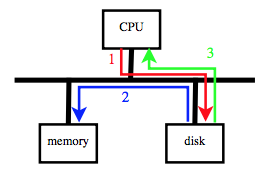
\includegraphics[scale=0.7]{pictures/dma.png}
\end{figure}
\begin{itemize}
  \item[1.] CPU issues DMA request to device
  \item[2.] Device directs data transfer
  \item[3.] Device interrupts CPU on completion
\end{itemize}


\newpage
\section{File Systems}
\subsection{Files and File Systems}
Files: persistent, named data objects
\begin{itemize}
  \item data consists of a sequence of numbered bytes
  \item file may change size over time
  \item file has associated meta-data. Ex., owner, access controls, file type, creation and access timestamps
\end{itemize}

\subsubsection{File Interface: Basics}
open
\begin{itemize}
  \item open returns a file identifier (or handle or descriptor), which is used in subsequent operations to identify the file
  \item other operations (e.g., read, write) require file descriptor as a parameter
\end{itemize}

close
\begin{itemize}
  \item kernel tracks while file descriptors are currently valid for each process
  \item close invalidates a valid file descriptor
\end{itemize}

read, write, seek
\begin{itemize}
  \item read copies data from a file into a virtual address space. \texttt{read(fileID, vaddr, length)}
  \item write copies data from a virtual address space into a file
  \item seek enables non-sequential reading/writing
\end{itemize}

get/set file meta-data

\subsubsection{File Position and Seeks}
Each file descriptor (open file) has an associated file position. \\

Read and write operations,
\begin{itemize}
  \item start from the current file position
  \item update the current file position
\end{itemize}

This makes sequential file I/O easy for an application to request. \\

Seeks (\texttt{lseek}) are used for achieve for non-sequential file I/O,
\begin{itemize}
  \item \texttt{lseek} changes the file position associated with a descriptor
  \item next read ore write from that descriptor will use the new position
\end{itemize}

\subsubsection{Directories and File Names}
A directory maps \emph{files names} (strings) to \emph{i-numbers}
\begin{itemize}
  \item an i-number is a unique (within a file system) identifier for a file or directory
  \item given an i-number, the file system can find the data and meta-data for the file
\end{itemize}

Directories provide a way for applications to group related files.

\begin{figure}[H]
  \vspace{-15pt}
  \centering
  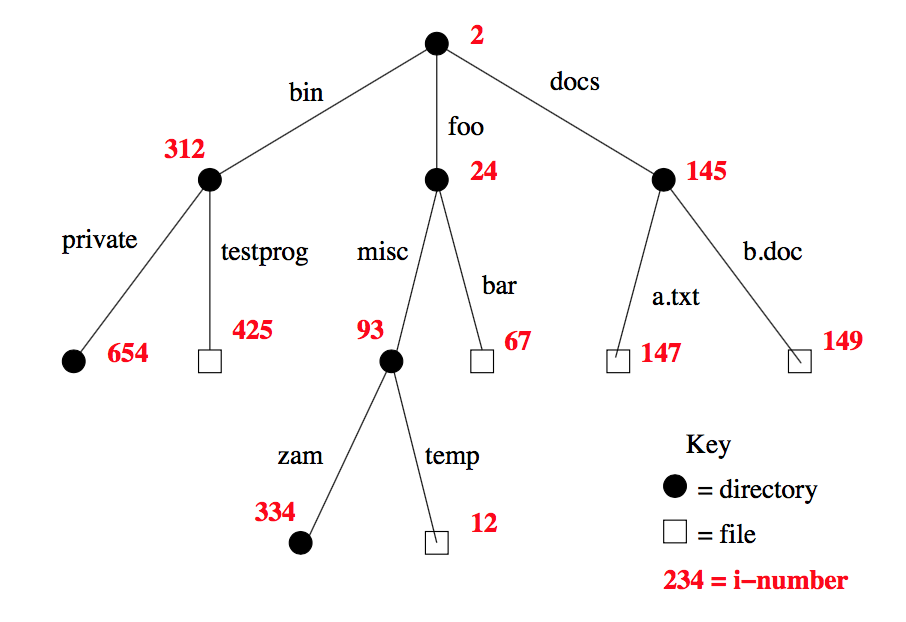
\includegraphics[scale=0.7]{pictures/directory_tree.png}
  \caption{Hierarchical Namespace Example}
  \label{fig:dir_tree_ex}
\end{figure}
Since directories can be nested, a file system's directories can be viewed as a tree, with a single \emph{root} directory.
In a directory tree, files are leaves. \\
Files may be identified by \emph{path names}, which describe a path through the directory tree from the root directory to the file.
Directories also have path names. \\
Applications refer to files using path names, not i-numbers.

\subsection{Links}
A \emph{hard link} is an association between a name (string) and an i-number. \\
Each entry in a directory is a hard link. \\

When a file is created, so is a hard link to that file; ex.,
\begin{itemize}
  \item \texttt{open(/foo/misc/biz, O\_CREAT|O\_TRUNC)}
  \item this creates a new file if a file called \texttt{/foo/misc/biz} does not already exist
  \item it also creates a hard link to the file in the directory \texttt{/foo/misc}
\end{itemize}

Once a file is created, \emph{additional} hard links can be made to it. \\
Ex., \texttt{link(/docs/a.txt, /foo/myA)} creates a new hard link \texttt{myA} in directory \texttt{/foo}.
The link refers to the i-number of file \texttt{/docs/a.txt}, which must exist. \\

Linking to an existing file creates a new path name for that file. \\
Each file has a \emph{unique} i-number, but may have \emph{multiple} path names. \\

Not possible to \texttt{link} to a directory (to avoid cycles)!

\subsubsection{Unlinking}
Hard links can be removed,
\begin{itemize}
  \item \texttt{unlink(/docs/b.doc)}
  \item this removes the link \texttt{b.doc} from the directory \texttt{/docs}
\end{itemize}
When the last hard link to a file is removed, the file is also removed! \\
Since there are no links to the file, it has no path name, and can no longer to opened.

\subsection{Multiple File Systems}
It is not uncommon for a system to have multiple file systems. \\

Some kind of global file namespace is required.
Examples,
\begin{itemize}
  \item \textbf{DOS/Windows}: use two-part file names: file system name, path name within file system.
  Example: \texttt{C:\\user\\cs350\\schedule.txt}

  \item \textbf{Unix}: create single hierarchical namespace that combines that namespaces of two file systems.
  Unix \texttt{mount} system call does this.
\end{itemize}

Mounting does \emph{not} two file systems into one file system,
\begin{itemize}
  \item it merely creates a single, hierarchical namespace that combines the namespaces of two file systems
  \item the new namespace is temporary --- it exists only until the file system in unmounted
\end{itemize}

\subsubsection{Unix mount Example}
\begin{figure}[H]
  \centering
  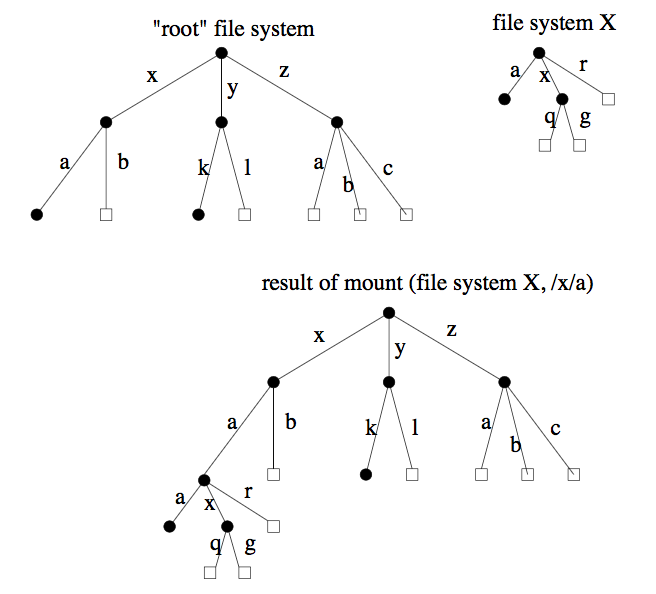
\includegraphics[scale=0.9]{pictures/unix_mount.png}
\end{figure}

\subsection{File System Implementation}
What needs to be stored persistently?
\begin{itemize}
  \item file data
  \item file meta-data
  \item directories and links
  \item file system meta-data
\end{itemize}

Non-persistent information,
\begin{itemize}
  \item open files per process
  \item file position for each open file
  \item \emph{cached} copies of persistent data
\end{itemize}

\subsubsection{File System Example}
Use an extremely small disk as an example:
\begin{itemize}
  \item 256 KB disk
  \item Most disks have a sector size of 512 bytes.
  Memory is usually \emph{byte addressable}.
  Disk is usually \emph{sector addressable}.
  \item 512 total sectors on this disk.
\end{itemize}

Group every 8 consecutive sectors into a block.
\begin{itemize}
  \item Better spatial locality (fewer seeks).
  \item Reduces the number of block pointers.
  \item 4 KB block is a convenient size for demand paging.
  \item 64 total blocks on this disk.
\end{itemize}

\subsection{i-nodes}
An i-node is a \emph{fixed-size} index structure that holds both file meta-data and a small number of pointers to data blocks. \\
i-node fields may include:
\begin{itemize}
  \item file type
  \item file permission
  \item file length
  \item number of file blocks
  \item time of last file access
  \item time of last i-node update, last file update
  \item number of hard links to this file
  \item direct data block pointers
  \item single, double, and triple indirect data block pointers
\end{itemize}

\subsection{VSFS: Very Simple File System}
Most of the blocks should be for storing user data (last 56 blocks).
\begin{figure}[H]
  \centering
  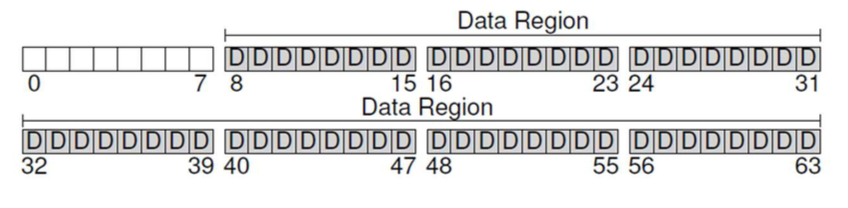
\includegraphics[scale=0.8]{pictures/vsfs_1.png}
\end{figure}

Need some way to map files to data blocks. \\

Create an array of i-nodes, where each i-node contains the meta-data for a file. \\
The index into the array is the file's index number (i-number). \\

Assume each i-node is 256 bytes, and we dedicate 5 blocks for i-nodes.
This allows for 80 total i-nodes/files.

\begin{figure}[H]
  \centering
  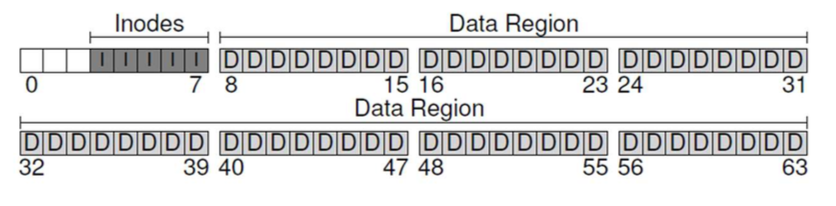
\includegraphics[scale=0.8]{pictures/vsfs_2.png}
\end{figure}

We also need to know which i-nodes and blocks are unused. \\
Many ways of doing this:
\begin{itemize}
  \item in VSFS, we use a bitmap for each.
  \item can also use a free list instead of a bitmap.
\end{itemize}

A block size of 4 KB means we can track 32K i-nodes and 32K blocks.
This is much more than actually required.
\begin{figure}[H]
  \centering
  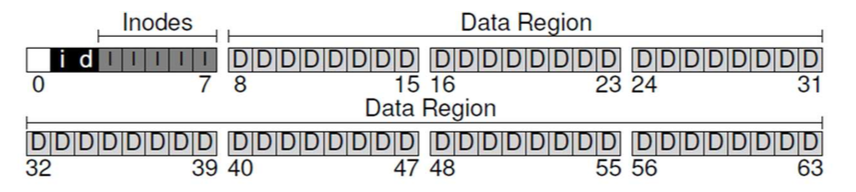
\includegraphics[scale=0.8]{pictures/vsfs_3.png}
\end{figure}

Reserve the first block as the \textbf{superblock}. \\
A superblock contains meta-information about the entire file system.
e.g., how many i-nodes and blocks are in the system, where the i-node table begins, etc.
\begin{figure}[H]
  \centering
  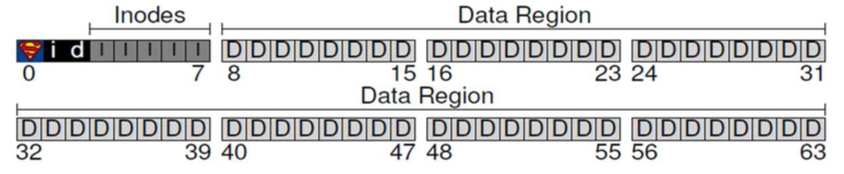
\includegraphics[scale=0.8]{pictures/vsfs_4.png}
\end{figure}
\begin{figure}[H]
  \vspace{-20pt}
  \centering
  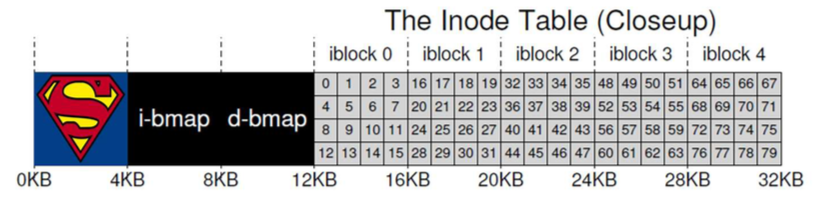
\includegraphics[scale=0.8]{pictures/vsfs_5.png}
\end{figure}

\subsubsection{VSFS: i-node}
Assume disk blocks can be referenced based on a 4 byte address. \\
$2^{32}$ blocks, 4 KB blocks.
Maximum disk size is 16TB. \\

In VSFS, an i-node is 256 bytes. \\
Assume there is enough room for 12 direct pointers to blocks. \\
Each pointer points to a different block for storing user data. \\
Pointers are ordered: first pointer points to the first block in the file, etc. \\

What is the maximum file size if we only have direct pointers? $12 \times 4$ KB $= 48$ KB. \\
Great for small files (which are common). \\
Not great if we want to store larger files.

\subsubsection{VSFS: Indirect Blocks}
In addition to 12 direct pointers, we can also introduce an \textbf{indirect pointer}. \\
An indirect pointer points to a block full of direct pointers. \\

4 KB block of direct pointers $=$ 1024 pointers. \\
Maximum file size is: $(12 + 1024) \times 4 \text{ KB} = 4144 \text{ KB}$ \\

What if the disk were larger? \\
Add a \textbf{double indirect pointer}, it points to a 4 KB block of indirect pointers. \\
Maximum file size is: $(12 + 1024 + 1024 \times 1024) \times 4 \text{ KB}$ (just over 4 GB).

\begin{figure}[H]
  \centering
  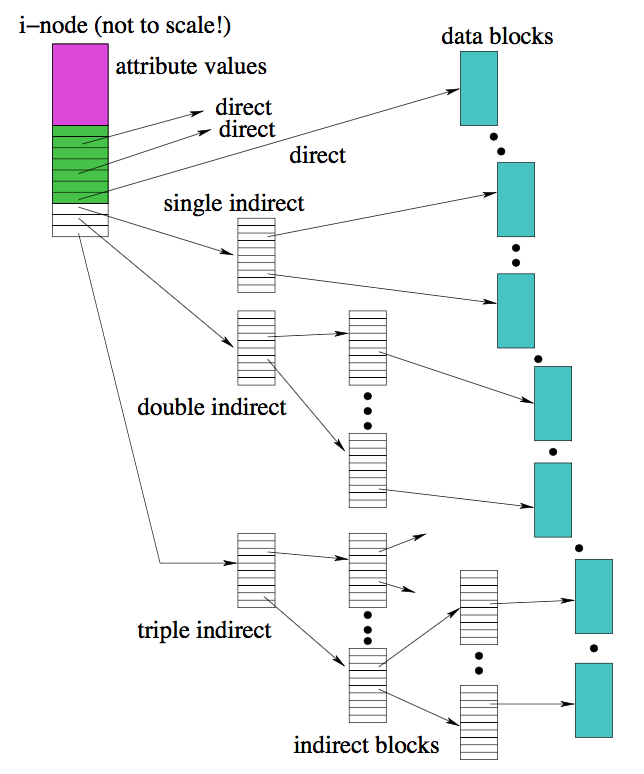
\includegraphics[scale=0.73]{pictures/i-node_diagram.png}
\end{figure}

\subsection{File System Design}
File system parameters:
\begin{itemize}
  \item \emph{How many i-nodes should a file system have?}
  \item \emph{How many direct and indirect blocks should an i-node have?}
  \item \emph{What is the ``right'' block size?}
\end{itemize}

For a general purpose file system, design it to be efficient for the common case,
\begin{table}[H]
  \centering
  \begin{tabular}{l|l}
  Most files are small & Roughly 2K is the most common size \\
  Average file size is growing & Almost 200K is the average \\
  Most bytes are stored in large files & A few big files use most of the space \\
  File systems contains lots of files & Almost 100K on average \\
  File systems are roughly half full & Even as disks grow, file system remains \textasciitilde50\% full \\
  Directories are typically small & Many have few entries; most have 20 or fewer
  \end{tabular}
\end{table}

\subsection{DIrectories}
Implemented as a special type of file. \\
Directory file contains directory entries, each consisting of a file name (component of a path name) and the corresponding i-number.
\begin{table}[H]
  \centering
  \begin{tabular}{l|l}
  name & i-number \\ \hline
  . & 5 \\
  .. & 2 \\
  foo & 12 \\
  bar & 13 \\
  foobar & 24
  \end{tabular}
\end{table}

Directory files can be read by application programs. \\
Directory files are only updated by the kernel, in response to file system operations. \\
Application programs cannot write directly to directory files.

\subsection{In-Memory (Non-Persistent) Structures}
\begin{itemize}
  \item per process
  \begin{itemize}
    \item descriptor table
    \begin{itemize}
      \item which file descriptors does this process have open?
      \item to which file does each open descriptor refer?
      \item what is the current file position for each descriptor?
    \end{itemize}
  \end{itemize}

  \item system wide
  \begin{itemize}
    \item open file table
    \begin{itemize}
      \item which files are currently open (by any process)?
    \end{itemize}
    \item i-node cache
    \begin{itemize}
      \item in-memory copies of recently-used i-nodes
    \end{itemize}
    \item block cache
    \begin{itemize}
      \item in-memory copies of data blocks and indirect blocks
    \end{itemize}
  \end{itemize}
\end{itemize}

\subsection{Reading from a File (/foo/bar)}
First, read the root i-node.
\begin{itemize}
  \item At ``well known'' position (i-node 2)
  \item i-node 1 is usually for tracking bad blocks
\end{itemize}
Read the directory information from root.
\begin{itemize}
  \item Find the i-number for foo
  \item Read the foo i-node
\end{itemize}
Read the directory information from foo.
\begin{itemize}
  \item Find the i-number for bar
  \item Read the bar i-node
\end{itemize}
Permission check. (is the user allowed to read this file?) \\
Allocate a file descriptor in the per-process descriptor table. \\
Increment the counter for this i-number in the global open file table. \\
Find the block using a direct/indirect pointer and read the data. \\
Update the i-node with a new access time. \\
Update the file position in the per-process descriptor table. \\
Closing a file deallocates the file descriptor and decrements the counter for this i-number in the global open file table.

\subsection{Problems Caused by Failures}
A single logical file system operation may require several disk I/O operations.

\begin{ex*}
Deleting a file,
\begin{itemize}
  \item remove entry from directory
  \item remove file index (i-node) form i-node table
  \item mark file's data blocks free in free space index
\end{itemize}
\end{ex*}

What if, due to a failure, some but not all of these changes are reflected on the disk?
\begin{itemize}
  \item System failure will destroy in-memory file system structures.
  \item Persistent structures should be \emph{crash consistent}, i.e., should be consistent when system restarts after a failure.
\end{itemize}

\subsubsection{Fault Tolerance}
Special-purpose consistency checkers (e.g., Unix \texttt{fsck} in Kerkeley FFS, Linux ext2),
\begin{itemize}
  \item runs after a crash, before normal operations resume
  \item find and attempt to repair inconsistent file system data structures, e.g.:
  \begin{itemize}
    \item file with no directory entry
    item free space that is not marked as free
  \end{itemize}
\end{itemize}

Journaling (e.g., Veritas, NTFS, Linux ext3),
\begin{itemize}
  \item record file system meta-data changes in a journal (log), so that sequences of changes can be written to disk in a single operation
  \item \emph{after} changes have been journaled, update the disk data structures (\emph{write-ahead logging})
  \item after a failure, redo journaled updates in case they were not done before the failure
\end{itemize}


\newpage
\section{Inter-process Communications and Networking}

\clearpage
\printindex
\end{document}

%%%%%%%%%%%%%%%%%%%%%
%% D O C U M E N T %%
%%%%%%%%%%%%%%%%%%%%%
